\chapter{ \label{chapter:il2} Methods to assess cell response to ex-vivo stimulation in flow cytometry }
%\chapter{ \label{chapter:il2} Effect of IL-2 Stimulation on Cell Phenotypes } 
%\chapter{ \label{chapter:il2} A recursive partitioning approach of identifying cells responsive to ex-vivo stimulation in flow cytometry }

%\epigraph{ {\fontfamily{frc}\selectfont \foreignlanguage{french} { Le Petit Prince, qui assistait à l'installation d'un bouton énorme, sentait bien qu'il en sortirait une apparition miraculeuse, mais la fleur n'en finissait pas de se préparer à être belle, à l'abri de sa chambre verte. Elle choisissait avec soin ses couleurs. }} }
\epigraph{ {\fontfamily{frc}\selectfont \foreignlanguage{french} { Mais la fleur n'en finissait pas de se préparer à être belle, à l'abri de sa chambre verte, elle choisissait avec soin ses couleurs. }} }

%In the previous chapter, I considered normalisation of the \gls{MFI} using beads, and replaced two univariate gating steps on CD25 and CD45RA.
Building on the work of the previous chapter, in which only two steps of the manual gating were replaced with an automatic algorithm, I will now consider a different dataset on which only preliminary manual analysis has been done.
In this chapter, I will revisit the bead normalisation method as well as elaborate on further normalisation methods, and will this time, attempt to replace the entire manual gating with a computational process.
In particular, I will develop approaches for discovering biologically relevant subsets not considered by the manual gating.

\section{Background}

\paragraph{Motivation}
%\Acrfull{GWAS}
Genomewide association studies have implicated the \cytokine{IL-2} signalling as an important aetiological pathway associated with the development of \gls{T1D}.  
%So far associated regions have been reported close to IL2RA and PTPN2, a phosphatase, which both influence STAT5 transduction.
%The protective rs12722495 haplotype was significantly associated with increase in CD25 expression on CD4 memory T cells measured in terms of MFI.
%Howevever the protective combined rs2104286 genotype led to a decrease in the percentage of CD25 positive CD4 naive T cells.  
As seen in \Cref{chapter:il2ra}, the protective T1D associated \gene{IL2RA} variant, at \snp{rs12722495} in healthy individuals, predicts an increase in the expression of \protein{CD25},
the alpha chain of the trimeric \protein{IL-2} receptor, on memory \protein{CD4}\positive T lymphocytes \citep{Dendrou:2008gc,Dendrou:2009dv}.
%and high levels of IL-2 secretion by these cells
%As supported by an increase in soluble CD25, this might be the consequence of preferential cleavage of the CD25 receptor \citet{Lowe:2007ij}.
%As supported by a decerase in soluble CD25 \citet{Lowe:2007ij}.
\citet{Garg:2012jr} found that regulatory and memory \protein{CD4}\positive T cells in healthy carriers of the T1D associated \snp{rs12722495} haplotype,
%T1D risk associated \gene{IL2RA} variants,
also exhibit decreased sensitivity to \cytokine{IL-2}.
The decreased sensitiviy was measured in terms of lower MFI levels of phosphorylated STAT5 (pSTAT5).
STAT5, the signal transducer and activator of transcription 5 protein, dimerises or tetramerises on phosphorylation and acts as a transcription factor that also induces the transcription of \gene{FOXP3}, one of the transcription factors characteristic of \glspl{Treg} (\Cref{figure:IL2-pathway}).

\begin{figure}[h]
\centering
\includegraphics[scale=.9]{figures/IL2-pathway.jpg}
\mycaption{figure:IL2-pathway}
{ Schematic of major IL-2 signaling pathway. }
{
    Figure from \citet{Liao:2013jt}.
    The trimeric \cytokine{IL-2} receptor (IL2R) is constituted of: the $\alpha$ chain \protein{IL2RA} (\protein{CD25}), the $\beta$ chain \protein{IL2RB} (\protein{CD122})
    and the $\gamma$ chain \protein{IL2RG} (\protein{CD132}).
    On binding of an \cytokine{IL-2} molecule to the receptor, a signalling cascade is initialised in which STAT5 is phosphorylated to pSTAT5, which then dimerises or tetramerises into a transcription factor.
    Cells express variable proportions of each of the components of the trimeric receptor with CD132 being the most commonly expressed.
    The pSTAT5 response to IL-2 is correlated with the relative expression of the three subunits.
    The pSTAT5 response is at its strongest when all three markers are highly expressed, intermediate when only CD25 and CD122 are expressed, and lower when only CD25 is present.
    Hence there is generally strong correlation between the \protein{CD25} MFI and the pSTAT5 MFI.
%IL2RB and \protein{IL2RA} makes up the intermediate affinity dimeric receptor, while IL2RA, IL2RB and IL2G make up the high affinity trimeric receptor.
%Schematic of Major IL-2 Signaling Pathways
%Shown is the activation of PI 3-K-AKT, JAK-STAT, and SHC-RAS-MAPK signaling pathways.
%Also shown are potential therapeutic points of control for IL-2 signaling, with anti-Tac (daclizumab), rapamycin, and JAK1 or JAK3 inhibitors being shown in red.
%The cartoon shows signaling by both STATs dimers and tetramers.
%The figure indicates that IL-2 activates more STAT5 than STAT3 and more STAT3 than STAT1. ERK refers to both ERK1 and ERK2. MEK refers to both MEK1 and MEK2.
}
\end{figure}

\citet{Long:2011hk} have reported that a \Gls{T1D} associated variant at \snp{rs1893217}
of the protein tyrosine phosphatase N2 gene (\gene{PTPN2}),
a negative regulator of the IL-2 pathway,
also correlates with lower pSTAT5.
%show diminished ability to respond to \cytokine{IL-2}.
Furthermore, it is suspected that \cytokine{IL-2} production might be diminished in T1D, since disease associated \gene{IL2RA} variants correlate with reduced CD25 levels and reduced \cytokine{IL-2} production on activated CD69\positive CD4\positive memory T cells after antigen stimulation \citep{Dendrou:2009dv}.
%with staphylococcal enterotoxin B 
%really?
Long-term reduced sensitivity to IL-2 also correlates with diminished maintenance of FOXP3 expression in the CD4\positive CD25\positive regulatory T cells of \gls{T1D} subjects \citep{Long:2010ej}.
%Defects in IL-2R signaling contribute to diminished maintenance 
%IL-2 sensitivity drives IL-2 stimulation
%Preliminary data also suggests that the sensitivity to IL-2, measured in terms of pSTAT5 activation, may be also be reduced in the regulatory CD4+ T cells of newly diagnosed T1D patients.
%Furthermore it is also suspected that IL-2 production might be diminished in T1D
%since disease associated variants in the \emph{IL2RA} and \emph{PTPN2} genotypes correlate with reduced IL-2 production (reference?). 
Hence, these findings appear to consolidate the hypothesis that type 1 diabetics tend to have a reduced ability to respond to IL-2
in part due to genetic differences in \gene{PTPN2}, \gene{IL2RA} and possibly other gene variants involved in the IL-2 signalling pathway
%and that this decreased sensitivity is most noticeable in regulatory T cells
\citep{Long:2010ej,Long:2011hk,Long:2012ea}.
%The cell subsets are not always consistently defined across studies.
%Long:2010ej define Tregs as CD4+ CD25hi (FOXP3 not measured)
%Long:2011hk report that CD4+ CD45RO+
%nor is the definition of response to IL-2
%sometimes pSTAT5 MFI is measured, sometimes pSTAT5 pct positive, sometimes pSTAT5 fold change
These results are of great clinical relevance to us, since our lab is currently conducting an adaptive study of IL-2 dose on regulatory T cells in type 1 diabetes (DILT1D\footnote{\url{http://www.clinical-trials-type1-diabetes.com/}}), and to all researchers interested in low-dose IL-2 therapy to autoimmune diseases \citep{Koreth:2011kv,Saadoun:2011em}.

However some concerns have been raised with these studies.
One concern was that the Tregs discrimination was not particulary thorough.
%nor consistent
\citet{Long:2010ej} define Tregs based only on two markers CD4\positive and CD25\positive, whereas these cells are usually also defined on CD127 and FOXP3.
Another a notable omission by \citet{Long:2010ej} was the lack of repeated samples to assess the within-individual variance or reliability of the assay.
%Although \citet{Long:2011hk} do assess repeatability in 16 individuals, its not accounted for in the association test.
%clinical trials which
%treat type 1 diabetics with IL-2.
In order to assess the validity of these results, \contributor{Tony Cutler}, in our lab, set to find if he could replicate some of these findings in an independent cohort, using a more refined gating stategy by including the FOXP3 regulatory T cell marker.
%T1D leads to decrease sensitivity to IL-2 in similar sample size with 
He also included the CD3 T cell marker, as well as more NK cell specific markers, CD8 and CD56,
%and the naive cell marker CD31,
to discover other cell subsets which may potentially, also be sensitive to IL-2 (\Cref{table:IL2-panels}).
%and using repeated samples.

\paragraph{Samples and panels}

He selected 22 long-standing diabetics (6 males and 16 females, mean age 29) and 28 controls (mean age 27) from the Cambridge Bioresource, as well as 30 newly diagnosed (20 males and 9 females, mean age 11.7) and 15 unaffected siblings of type 1 diabetics (5 males and 12 females, mean age 12.3) from the \Gls{D-GAP} resource.  
These were matched on age and sex to 43 controls.
%This was to determine if there was a difference between newly diagnosed and long-standing diabetics while controlling for age.
%To guard from false positive association and non-reproducible results, it is important to ascertain the repeatability of these cell phenotypes before conducting any form of association study.
%Before proceeding with association testing of these cell phenotypes with T1D status or other covariates,
In order to assess the reproducibility, ten individuals, five cases and five controls, were recalled for a second blood sample from the Cambridge Bioresource (\Cref{table:IL2-recalled-individuals}).

\begin{table}[ht]
\centering
\begin{tabular}{lllc}
  \hline
Individual & status  & pch & number of days between visits \\
  \hline
1          & control & a   & 98 \\
2          & case    & b   & 140 \\
3          & control & c   & 167 \\
4          & control & d   & 98 \\
5          & case    & e   & 167 \\
6          & case    & f   & 112 \\
7          & control & g   & 112 \\
8          & case    & h   & 98 \\
9          & case    & i   & 120 \\
10         & control & j   & 140 \\
   \hline
\end{tabular}
\mycaption{table:IL2-recalled-individuals}
{Ten individuals recalled between 98 and 168 days later to assess stability of the cell phenotypes. }
{
pch is the plotting character used to refer to these individuals in plots later in this chapter.
}
\end{table}
%In order to test these hypotheses, we selected 21 long-standing diabetics and 30 controls from the Cambridge Bioresource,
%as well as  28 newly diagnosed and 14 unaffected siblings from DGAP.
%The nature of the resource allows more flexibility to recall patients of interest, i.e those with low IL-2 signalling potential, for more in depth analysis.
%To test this hypothesis, blood samples are taken from 21 type 1 diabetics and 30 healthy controls.  
Blood samples were prepared and analysed by flow cytometry on day of collection.
Each sample was split into four aliquots of \SI{500}{\micro\litre}.
The first aliquot was left unstimulated.
The remaining three were stimulated ex-vivo for 30 minutes at four 100-fold increasing doses
of proleukin, a polymer of \cytokine{IL-2}, at $0.1$, $10$ and \SI{1000}{\unit\per\milli\litre} respectively.
%\SI{1000}{\unit\per\micro\litre} respectively.
After the set stimulation time, the samples were fixed, permeabilised and stained, with different panels (\Cref{table:IL2-panels}), 
on a set of core markers, not expected to be affected by short-term proleukin stimulation,
CD4, CD25, CD45RA and FOXP3.
These were used to delineate different cell types, and the functional marker, pSTAT5,
%a signalling protein of the IL-2 pathway phosphorylated on IL-2 stimulation (\Cref{figure:IL2-pathway}),
was used to measure proleukin response.
In order to control for batch, age or sex, \gls{T1D} samples were, when possible, ran in parallel with an age and sex paired healthy control, although in practice, this was not always possible (\Cref{figure:IL2-sample-time}).
Also for practical and financial reasons, not all samples were stained with every panel (\Cref{table:IL2-panels}).
Hence the case-control statistical analysis was only conducted in samples stained with the CD4 T cell panel, which included all samples in the study.

%We address the following research questions relating to the pSTAT5 response in these samples:
%\begin{itemise}
  %%\item Can some individuals be classified as low/high responders?
  %\item In the cell subsets identified by manual gating, is the response to IL-2 associated with case-control status or any other covariate? 
  %\item Using automated methods, can we find other responsive cell subsets which are ignored by the manual gating?
%\end{itemise}
%Answering the first question will depend on the reproducibility of the response between cell-subsets within individuals,
%and we will see if, as in \Cref{chapter:il2ra}, normalisation can improve the reproducibility.

%Tony Cutler, Saleha Hassan, Marcin Pekalski will be involved in immune function assays.
%Louise Bell will be ethics liason.
%Statistical analysis will be carried out by a delegated member of the Statistics team.
%Demands on DIL infrastructure 
%Blood handling rooms, BD LSRII Fortessa machine.  

\begin{table}[h!]\footnotesize
\centering
\begin{tabularx}{.6\textwidth}{lcc}
\rowcolor{Gray}
Flurochrome       & T/NK cell panel & CD4 T cell panel   \\
Alexa Fluor 488   & pSTAT5          & pSTAT5             \\
Alexa Fluor 700   & CD4             & CD4                \\
APC               & CD25            & CD25               \\
Pacific Blue      & CD56            & CD45RA             \\
PE YG             & FOXP3           & FOXP3              \\
PE-Cy7 YG         & CD45RA          &                    \\
PerCP Cy5-5       & CD3             &                    \\
Qdot 605          & CD8             &                    \\
\hline
Number of samples &  5              & 95               \\
%Number of samples & 13 & 96 &
\end{tabularx}
\mycaption{table:IL2-panels}
{Proleukin stimulation assay antibody-fluorochrome panels.}
{
The fluorochrome-antibody panels used in IL-2 stimulation.
The panel used on the majority of samples was the CD4 T cell panel, used to disriminate
effector and regulatory naive and memory T cells.
The T/NK cell panel, which contains the most markers, was only ran on a subset of 5 samples.
}
\end{table}

%\begin{table}[h!]\footnotesize
  %\centering
%\begin{tabularx}{\textwidth}{lcccc}
%\rowcolor{Gray}
%Flurochrome       & T/NK cell panel & CD4 T cell panel & CD4/naive cell panel & NK cell panel \\
%Alexa Fluor 488   & pSTAT5          & pSTAT5           & pSTAT5               & pSTAT5  \\
%Alexa Fluor 700   & CD4             & CD4              & CD4                  & CD4     \\
%APC               & CD25            & CD25             & CD25                 & CD25    \\
%Pacific Blue      & CD56            & CD45RA           & CD45RA               & CD45RA  \\
%PE YG             & FOXP3           & FOXP3            & FOXP3                & FOXP3   \\
%PE-Cy7 YG         & CD45RA          &                  & CD31                 & CD56    \\
%PerCP Cy5-5       & CD3             &                  &                      & \\
%Qdot 605          & CD8             &                  &                      & \\
%\hline
%Number of samples &  5              & 95               & 12                   & 66 \\
%%Number of samples & 13 & 96 &
%\end{tabularx}
%\mycaption{table:IL2-panels}
%{Proleukin stimulation assay antibody-fluorochrome panels.}
%{
%The fluorochrome-antibody panels used in IL-2 stimulation.
%The panel used on the majority of samples was the CD4 T cell panel, used to disriminate
%effector and regulatory naive and memory T cells.
%The T/NK cell panel, which contains the most markers, was only ran on a subset of 5 samples.
%}
%\end{table}


%CD14-CD19-CD3-CD45RA-CD56-HLA-DR-PSTAT5
%1
%CD19-CD25-CD27-CD3-CD45RA-CD56-CD8-PSTAT5
%1
%CD19-CD25-CD27-CD3-CTLA4-PSTAT5
%1
%CD19-CD25-CD27-CD3-ISO-PSTAT5
%1
%CD25-CD31-CD4-CD45RA-FOXP3-PSTAT5
%5
%CD25-CD3-CD4-CD45RA-CD56-CD8-CD8-PSTAT5
%1
%CD25-CD3-CD4-CD45RA-CD56-CD8-FOXP3-PSTAT5
%13
%CD25-CD3-CD4-CD45RA-CD56-CD8-PSTAT5
%48
%CD25-CD3-CD4-CD45RA-CD56-FOXP3-PSTAT5
%37
%CD25-CD4-CD45RA-CD56-FOXP3-PSTAT5
%5
%CD25-CD4-CD45RA-FOXP3-KI67-PSTAT5
%1
%CD25-CD4-CD45RA-FOXP3-PSTAT5
%50
%
%\begin{figure}
%\centering
%\includegraphics[scale=.5] {flowdatasets/figures/il2-stimulation-samples-time.pdf}
%\mycaption{figure:IL2-sample-time} 
%{ Days on which samples are processed. }
%{
  %To account for day of analysis effect in the case-control association testing,
  %at least one healthy control sample and one type 1 diabetic sample were analysed per day.
%}
%\end{figure}

\myfigure{scale=.6}{IL2-sample-time} 
{ Number of cases and controls analysed per day in the 95 samples. }
{
  To account for batch effects in the case-control association testing,
  Tony Cutler aimed to analyse, when possible,
  at least one healthy control sample and one type 1 diabetic sample per day.
  %However on some days the number of cases and controls did not match.
  However, on two days, 2012-09-04 and 2012-10-25, no matching controls were run.
}

\clearpage

\section{Preliminary analysis by Tony Cutler}

In this section, I will describe the preliminary manual analysis using FlowJo that was conducted by \contributor{Tony Cutler}.
%The pSTAT5 distribution was measured in effector and regulatory naive and memory T cell populations (Figure~\ref{figure:tony-cd4-gating}).
Four CD4\positive lymphocyte subsets (\Cref{figure:tony-cd4-gating}) were gated manually using FlowJo:
\begin{itemise}
    \item memory effector T cells (Teffs)
    \item memory regulatory T cells (Tregs)
    \item naive Teffs
    \item naive Tregs
\end{itemise}
%\begin{figure}[h]
    %\centering
    %\includegraphics[scale=.75]{figures/tony-cd4-gating.pdf}
    %\caption{  \label{figure:tony-cd4-gating} Manual gating conducted by \contributor{Tony Cutler} to identify:
    %conventional and regulatory naive and memory T cells as well as activated regulatory T cells.
    %}
%\end{figure}

%\hspace{-2cm}
\begin{figure}[h]
\centering
  \includegraphics[scale=.75]{figures/CB00366X_2012-11-07.pdf}
\mycaption{figure:tony-cd4-gating}
{Gates applied across doses.}
{
Manual gating conducted using FlowJo by \contributor{Tony Cutler} to identify
naive Teffs (green ellipse) and Tregs (blue ellipse) (e)
and memory Teffs (black ellipse) and Tregs (red ellipse) (f).
%The same gates can be applied across doses (i, ii, ,iii, iv).
}
\end{figure}

Within each lymphocyte subset, the pSTAT5 distribution was measured, in each of the four samples stimulated at an increasing proleukin dose
(\Cref{figure:dose-effect-pstat5-cellsubsets-density}).  
As expected, the pSTAT5 distribution shifts progressively right for higher doses of proleukin, as more STAT5 is phosphorylated.
Of the four subsets, the most sensitive cells to proleukin are the rarer memory and naive Treg subsets (\Cref{figure:dose-effect-pstat5-cellsubsets-density} b and d),
then the memory Teffs (\Cref{figure:dose-effect-pstat5-cellsubsets-density} a) and finally the naive Teffs (\Cref{figure:dose-effect-pstat5-cellsubsets-density} c).
This correlates with the level of \protein{CD25} expressed by these cells.

%\includegraphics[scale=.45]{figures/dose-effect-pstat5-cellsubsets-density.pdf}
%\includegraphics[scale=.45]{figures/dose-effect-pstat5-cellsubsets-density-baseline.pdf}
%\includegraphics[scale=.45]{figures/dose-effect-pstat5-cellsubsets-ecdf-joined.pdf}
\myfigureh{scale=.6}
%individual g
{dose-effect-pstat5-cellsubsets-density}
{ pSTAT5 distribution in the manually gated cell subsets from \Cref{figure:tony-cd4-gating}. }
{
The thickness of the lines is representative of the four increasing doses of proleukin (0, 0.1, 10 and 1000 units).
The dose-response is most striking in the smaller Treg subsets with higher CD25 (b and d).
The dashed vertical line represents the 99th percentile of the pSTAT5 distribution in the resting sample,
which is used to define the pSTAT5\positive threshold.
}

Next the repeatability of the pSTAT5 response was assessed by measuring the pSTAT5 \gls{MFI} in each of the four subsets.
This pSTAT5 response cell phenotype was poorly reproducible, since the location of the peaks was not stable across days as illustrated by the sample shown in \Cref{figure:dose-effect-pstat5-cellsubsets-density-repeatability}.
%Furthermore, the \gls{MFI} is not a representative metric for bimodal distributions 
%However, one issue is that pSTAT5 MFI is not very representative for very bimodal or skewed distributions such
%as the memory Teffs in \Cref{figure:dose-effect-pstat5-cellsubsets}.
%Also the resting pSTAT5, which represents the baseline pSTAT5, of the same cell subset may not be constant across days.  
%To address these issues, the percent of pSTAT5\positive cells was also assessed.
\myfigureh{scale=.6}
%individual g
{dose-effect-pstat5-cellsubsets-density-repeatability}
{ pSTAT5 distribution in an individual on visit one (black) and visit two (red).
}
{
In black, the pSTAT distribution on visit one and in red, on visit two.
%The thickness of the line represents the proleukin dose at which the sample was stimulated (0, 0.1, 10 and 1000 units).
The thinner lines are from the resting sample whereas the thicker lines are from the sample stimulated at 1000 units.
The vertical lines represent the pSTAT5\positive threshold set at the $99^{th}$ percentile of the pSTAT5 distribution in the resting sample.
This clearly shows that pSTAT5 distribution is not stable across days in the four cell subsets.
}
This motivated a threshold approach to define the ratio of cells which are pSTAT5\positive.
An idea similar to that applied in \Cref{chapter:il2ra} to define naive cells as CD25\positive.
%but the threshold is defined using the unstimulated sample rather than beads. 
%It is a good approach to use when the number of cells is small
%and is commonly used in populations with high CV.
However, here an internal threshold was used, namely
the threshold was defined to be the 99th percentile of the pSTAT5 distribution in the resting cell subset per sample.
Thus each each sample and cell subset had its own pSTAT5\positive threshold.
He presented his results in six of the ten repeated individuals for the four stimulated cell subsets,
memory Teffs (\Cref{figure:tony-memory-eff}),
memory Tregs (\Cref{figure:tony-memory-treg}),
naive Teffs (\Cref{figure:tony-naive-eff})
and naive Tregs (\Cref{figure:tony-naive-treg}).
For memory and naive Tregs (\Cref{figure:tony-memory-treg,figure:tony-naive-treg}), at the highest 1000 units dose,
practically all memory and naive Tregs are pSTAT5\positive.
However, these cell populations show a significant response already at the lowest 0.1 units dose of proleukin.
Based on this observation, the memory and naive Treg pSTAT5 cell phenotype was selected to be the percentage of pSTAT5\positive cells at the 0.1 units dose.
On the other hand, since memory Teffs are less responsive, 10 units was chosen as the representative dose.
For naive Teffs, the least responsive of the four cell subsets considered, the repeatability was assessed at the 1000 unit dose.
The repeatability was assessed with the coefficient of determination:
%instead of using the square of the Pearson correlation: 
\[
  R^2 = 1 - \frac{\sum_{i=1}^N (x_{i1}-x_{i2})^2}{\sum_{i=1}^N (x_{i1}-\overline{x_1})^2}
\]
where $x_{i1}$ is the phenotype of $i^{th}$ individual on the first day and $x_{i2}$
is the phenotype of the $i^{th}$ individual on the second day.
The coefficient of determination can take negative values if the correlation between $x_{i1}$ and $x_{i2}$ is very low.
Contrary to the Pearson correlation, used in the previous chapter, the coefficient of determination is sensitive to linear transforms.
%this is not correct because it's not symmetric
In \Cref{figure:tony-repeatability}, even when using the percent of pSTAT5\positive cell phenotype, the overall reproducibility across the four cell subsets was still poor, with the more sensitive and smaller cell subsets, naive and memory Tregs showing the worst correlation ($R^2=-0.16$ and $R^2=-0.82$), memory Teffs showing slightly better correlation ($R^2=0.021$) and finally the less responsive naive Teffs showing good correlation ($R^2=0.7728$).
The association with \gls{T1D} was tested using a two-tailed paired t-test of 20 cases matched with 20 controls analysed on the same day (\Cref{figure:tony-t1d-association}).
%how did he deal with repeats?
He also tested for association with \gene{IL2RA} SNP \snp{rs12722495}, and the
\gene{PTPN2} SNPs \snp{rs45450798} and \snp{rs478582} (plots not shown).
No significant association was detected either with disease or with genotype.


\begin{figure}
\centering
%
\begin{minipage}{.65\textwidth}
\includegraphics[width=\linewidth]{figures/tony-memory-eff}
\end{minipage}
\begin{minipage}{\textwidth}
\mycaption{figure:tony-memory-eff}
{ The percentage of pSTAT5\positive cells increases with proleukin dose in memory Teffs.  }
{
    Plot produced by Tony Cutler.
    The percent of pSTAT5\positive cells increases with proleukin dose in memory Teffs, but the measured response is not consistently repeatable (f, g).
}
\end{minipage}
%
\begin{minipage}{.65\textwidth}
\includegraphics[width=\linewidth]{figures/tony-memory-treg}
\end{minipage}
\begin{minipage}{\textwidth}
\mycaption{figure:tony-memory-treg}
{ The percentage of pSTAT5\positive cells increases with proleukin dose in memory Tregs. }
{
  Plot produced by Tony Cutler.
  While at the highest proleukin dose of 10 and 1000 units, all memory tregs are consistently pSTAT5\positive,
  there is more discrepancy at the low dose of 0.1 units.
}
\end{minipage}
\end{figure}


\begin{figure}
\centering
\begin{minipage}{.65\textwidth}
\includegraphics[width=\linewidth]{figures/tony-naive-eff}
\end{minipage}
\begin{minipage}{\textwidth}
\mycaption{figure:tony-naive-eff}
{ The percentage of pSTAT5\positive cells increases with proleukin dose in naive Teffs. }
{
  Plot produced by Tony Cutler.
  Only \pct{40} of the naive effector cells are pSTAT5\positive even at the highest 1000 unit proleukin dose.
}
\end{minipage}
\begin{minipage}{.65\textwidth}
\includegraphics[width=\linewidth]{figures/tony-naive-treg}
\end{minipage}
\begin{minipage}{\textwidth}
\mycaption{figure:tony-naive-treg}
{ The percentage of pSTAT5\positive cells increases with proleukin dose in naive Tregs. }
{
  Plot produced by Tony Cutler.
  While at the highest proleukin doses of 10 and 1000 units, all naive tregs are consistently pSTAT5\positive,
  there is more discrepancy at the low dose of 0.1 units.
}
\end{minipage}
\end{figure}

\begin{figure}
\centering
\begin{minipage}{.65\textwidth}
\includegraphics[width=\linewidth]{figures/tony-repeatability}
\end{minipage}
\begin{minipage}{\textwidth}
\mycaption{figure:tony-repeatability}
{ Repeatability of pSTAT5\positive in six individuals in the four cell subsets. }
{
    Plot produced by Tony Cutler.
    The repeatability of the percent of cells which are pSTAT5\positive is assessed in effector memory and naive at the 10 units and 1000 units dose respectively, and in memory and naive Tregs at the 0.1 units dose.
    While the repeatability in the naive effector subset was good ($R^2=0.7728$), the repeatability in the other cell subsets is poor (memory Teffs $R^2=0.021$, naive tregs $R^2=-0.16$ and memory tregs $R^2=-0.82$).
}
\end{minipage}
\begin{minipage}{.65\textwidth}
\includegraphics[width=\linewidth]{figures/tony-t1d-association}
\end{minipage}
\begin{minipage}{\textwidth}
\mycaption{figure:tony-t1d-association}
{ Association test of percent pSTAT5\positive in the four cell subsets. }
{
  Plot produced by Tony Cutler.
  The association with T1D of the percent of cells which are pSTAT5\positive is assessed in effector memory and naive at the 10 units and 1000 units dose
  respectively, and in memory and naive Tregs at the 0.1 units dose.
  The association test is a two-tailed paired-t-test on 20 cases paired with 20 controls analysed on the same day (40 out of the available 96 individuals).
  No significant association is detected.
}
\end{minipage}
\end{figure}

%\section{Automatic methods}
%\subsection{Normalisation of pSTAT5 improves repeatability}
\section{Reproducibility of pSTAT5 response within an individual}

\contributor{Tony Cutler}'s preliminary results in the six repeated individuals suggested that the pSTAT5 MFI and percent pSTAT5\positive were poorly reproducible
cell phenotypes using the methodology and approach described, which consequently would give us little power to detect an association with disease status or genetics.
In \Cref{chapter:il2ra}, repeatability of CD25 MFI in memory cells was improved thanks to bead normalisation.
This motivated me to see whether on this data, normalisation approaches would also improve the repeatability of these cell phenotypes.
%Furthermore, since these cell phenotypes were only defined at a single dose, I also defined new cell phenotypes to summarise the response across doses.
%This suggests that variation in the instrument is not the main cause of variation in the data and therefore that bead normalisation cannot be usefully applied.

\subsection{Normalisation approaches}

\paragraph{Bead normalisation} 
In \Cref{chapter:il2ra}, I used beads to correct for day to day variation in the CD25 channel.
However for these data, using beads in the Alexa-488 channel, the fluorochrome conjugated to pSTAT5 (\Cref{table:IL2-panels}),
%\Cref{chapter:il2ra}
did not adequately capture the short term variation in pSTAT5 (\Cref{figure:pstat5-beads}).  
%This suggests that for this experiment, flurorescent beads do not explain the day to day variation in the pSTAT5 MFI.
This suggests that day to day variation in the instrument is unlikely to be the major cause of day to day variation in the data, and that bead normalisation cannot be usefully applied.

\paragraph{ Correcting for baseline MFI }
One observation which can be drawn from \Cref{figure:dose-effect-pstat5-cellsubsets-density-repeatability} is that the
MFI of the pSTAT5 distribution in the resting sample is different across days.
If a cell population had a higher resting pSTAT5 MFI due only to day to day variability,
then one might expect that the pSTAT5 MFI in the stimulated population would also be higher.
%First I noticed that Tony had not corrected for baseline MFI.
I first attempted to account for the difference in resting pSTAT5 by
taking the ratio of the MFI of the stimulated populations over that of the MFI of the resting population,
or equivalently by subtracting the log transformed MFIs.
%subtracting the MFI of the resting population from the MFI of the stimulated populations.
%Since fluorescence intensity scales multiplicately, I also attempted to do the correction by dividing by the baseline MFI
%or alternatively by subtracting the log transformed MFIs.
However, this did not appear to improve the repeatability significantly but instead just reduced the MFI by the same factor on both days
(\Cref{figure:pstat5-mfi-cellsubsets-repeatability}).
This suggests that the day to day variation in the resting sample MFI does not capture the variation in the stimulated population
.

\begin{figure}
\centering
\begin{minipage}{.8\textwidth}
\includegraphics[width=\linewidth]{figures/pstat5-beads}
\end{minipage}
\begin{minipage}{\textwidth}
\mycaption{figure:pstat5-beads}
{Variation in pSTAT5 MFI is not captured by variation in bead MFI.}
{
  For the purpose of MFI normalisation, the fluorescence intensity of six-peak flow cytometry beads
  was measured in the Alexa 488 channel, the fluorochrome conjugated to the pSTAT5 marker.
  However, as illustrated by the loess lines, the MFI of the three dimmest populations of beads (orange)
  does not capture the pSTAT5 MFI time variation in the four cell subsets.
  The pSTAT5 MFIs are obtained from samples stimulated at 1000 units of proleukin.
  
}
\end{minipage}
\end{figure}


\paragraph{\label{paragraph:ANN} Nearest-neighbour joining}
%While using a different background MFI should account for differences in resting MFI,
%this assumes that the MFI difference is representative of the pSTAT5 shift.
%This may not be true for distributions which change modality.
One concern with adjusting by baseline MFI is that differences in cell counts across samples stimulated at different doses, may influence the accuracy of the MFI estimate.
Another concern is that since the pSTAT5 distribution is often bimodal in the cell populations considered, substracting the MFI may not be ideal.
Instead, a more correct approach would be to subtract the pSTAT5 fluorescence intensity for each resting cell.
One way of emulating this is to match each cell to its closest neighbour in the unstimulated sample.  
This was accomplished by joining samples on their core markers using the \gls{ANN} to the resting sample \citep{Jones:2011ez}
as implemented in the \Rpackage{RANN}.
This created a dataset of the same number of cells as the resting dataset, but where each cell now had a total of four functional pSTAT5 markers,
one for each stimulation dose.
At each cell it is now possible to assess the difference in pSTAT5 response between resting and stimulated states.
This is important because cells do not all have the same resting level of pSTAT5 (\Cref{figure:pstat5-baseline-relative}).
This approach presents a number of advantages.
Firstly, only the sample to which the other samples are joined needs to be gated.
Secondly, since the pSTAT5 response is relative to the baseline, it should be more robust to variation between days
and consequently, more reproducible than pSTAT5 fluorescence intensity.
Thirdly, since we have response at the cell-level, we can apply methods
%such as \gls{CART}, \gls{RF} or \gls{MARS}
to do multivariate regression of pSTAT5 from core markers.
This could help identify cells which would have been missed from only examining core markers.
%However, even when we correct for the different baseline, the distance between the peak of the resting sample and the stimulated sample is not constant
%An advantage of this method is that number of cells per cell type is constant across doses.
%A disadvantage of this method is that the number of cells is very different of that all the cells are shifted then they will all be joined to closest neighbour
%which could be a single point.
%which will investigate in the second section.
%An alternative to this approach, would be to gate subsets in subsamples stimulated at different doses and subtract the background,
%however a clear advantage of this approach is that it allows for methods such as RF and MARS
The \gls{ANN} approach is valid without normalisation since the distributions of the core markers align across doses.
%(\Cref{figure:core-markers}).
%\Cref{figure:ann-join-0 units-01 units} confirms that the mapping of the clusters is correct across the nearest-neighbour mapping.
%When the between-dose variation on the core markers is negligeable,
%If we assume that the within-tube variation is negligeable, then a simpler solution is possible:
%each cell in the unstimulated subsample is joined to its closest neighbouring cell (in terms of its core markers) in a stimulated subsample.
%This assumes that the core markers are fairly stable across samples, which is usually the case in ex-vivo stimulated.
%The joining results is also not affected by any euclidean distance preserving transform, so the FCS data can be transformed before or after the \gls{ANN} joining.
%Another important check is to see whether the joining is sensitive to the transform.
%We find that we get the same results whether we join before or after the transform.
%\myfigure{scale=.3}{dose-effect-core-markers}{Dose-effect on core markers in ungated sample.} { Increasing doses represented by lines of increasing thickness.  The distributions align well across doses.  }
However, using this nearest-neighbour joining method, the repeatability of the cell phenotypes pSTAT5 MFI (\Cref{figure:nn-pstat5-mfi-cellsubsets-repeatability}) and the percent of pSTAT5\positive (\Cref{figure:pstat5-pos-cellsubsets-repeatability}) are not substantially improved.

%
%\myfigure{scale=.3}{ann-join-0 units-01 units}
%{ Nearest neighbour join on core markers of ungated resting sample with ungated sample stimulated at 0.1 units. }
%{
%All clusters lie on the y=x line which suggests that the largest clusters are correctly matched across samples.
%}
%

\begin{figure}
\centering
\begin{minipage}{.8\textwidth}
\includegraphics[width=\linewidth]{figures/pstat5-baseline-relative}
\end{minipage}
\begin{minipage}{\textwidth}
\mycaption{figure:pstat5-baseline-relative}
{ pSTAT5 intensity across the four proleukin doses, before (a) and after (b) per-cell baseline pSTAT5 subtraction in the ungated sample.}
{
  An important proportion of cells are already saturated for pSTAT5 (high baseline) in the resting sample (a).
  Correcting for the per cell pSTAT5 baseline, shows the true proportion of cells which responds to proleukin within this sample (b).
}
\end{minipage}
\end{figure}

\paragraph{Peak alignment}
%The repeatability of the pSTAT MFI was assessed.  
Another approach to the normalisation as implemented in the \Rpackage{flowStats}, is to align the modes of the distributions across days in the ungated sample.
The method assumes that the two peaks in the pSTAT5 distribution, representing stimulated and unstimulated cells, should exist in all ungated samples, while their locations and their proportions may vary across doses and days.
%Given that the location of the peaks of pSTAT5 in the ungated sample remains fairly stable across doses but that the heights vary,
%this advocates a normalisation method which relies on peak alignment.
%If we expect that the core cell populations should exist in all samples but that their locations and their proportions may vary across days and dose,
%a normalisation approach is to align the location of the population across doses per day.
%Hence we wish to align the location of the peaks across days while allowing for the relative proportion of the populations to vary.  
%The idea is to identify the groups based on a single marker by clustering algorithm and then selecting the peaks to be the group medians.
%In this approach the number of groups K needs to be known a priori and is assumed to be the same across samples.
%This is the method used by \Rpackage{flowBeads} which identifies groups with the k-medoids algorithm for the purpose of bead normalisation.
%In Chapter 3, I used k-means to identify the peaks, but I found on this data k-means and k-medoids performed poorly since the cluster variances are very different.  
Unfortunately in flow cytometry, the peaks are not always clearly identifiable due to noise associated with staining.
This is particularly noteable in ungated data where debris obfuscate the pSTAT5 signal and can introduce artefactual peaks, leading to peak misidentification.
Furthermore, the transform can also introduce spurious peaks close to zero.
In particular, the second peak corresponding to the stimulated cells is much broader and smaller since the majority of cells in the sample are not stimulated.
However I found that upon gating on lymphocytes and CD4\positive lymphocytes, these spurious peaks disappear and both peaks were correctly identified.
%A mixture model algorithm would be better suited since it allows for different variances in the clustering.
%but because of the skewness of the data, the peaks did not correspond to the cluster medians.
To identify the peaks, I used a sliding window approach on the density function.
The sliding window records the point with the highest density estimate in the current window,
so that within a window of twice the span, the point of highest density is selected as a peak.
At the end, a list of highest density points is returned of which the top two are selected.
I found in practice this method worked well with a window span of $40$ across all samples considered.
%This approach is useful for estimating K but the window size may need to be tuned per sample.  
%depending on the value of the width parameter selected for the logicle transform.
%(\Cref{appendix:transformation,appendix:normalisation}).
(\Cref{figure:pstat5-peak-normalisation}).
\begin{figure}[h]
    \centering
    \includegraphics[scale=.5]{figures/pstat5-peak-normalisation.pdf}
    \mycaption{figure:pstat5-peak-normalisation}
    {Normalisation by peak alignment of the pSTAT5 distribution in lymphocytes (a and b) and CD4\positive lymphocytes (c and d).}
    {
      The two peaks of the pSTAT5 distribution are identified using a sliding window approach,
      in the lymphocyte sample stimulated at 1000 units (a) and in the manually gated CD4\positive lymphocyte subset stimulated at 10 units (c).
      In the normalised pSTAT5 distribution in the ungated (a) and CD4\positive lymphocyte subset (d),
      the identified peaks in (a) and (c) have been mapped to the respective medians across all peaks.
    }
\end{figure} 
In order to facilitate peak identification in the CD4\positive lymphocytes, I considered the pSTAT5 distribution at 10 units instead of 1000 units, since the unstimulated to stimulated ratio is more even at an intermediate dose.
%since at the highest dose, most CD4\positive lymphocytes are stimulated.
%Here's an example of this method applied on simulated data where the number of peaks is known and easily identifiable (Figure~\ref{figure:simulation-peak-align}).
%The sliding window method is good for detecting local maximums while the clustering approach is better at find global splits.
%Hence we combine both approaches by using the sliding window on the partitions identified by the clustering.
%We apply mclust and pam (clara) because mclust tends to the fit the data better when the cluster are of very uneven size like example (~/pam.fail.RDAta).
Once the two peaks were identified in all samples,
%the next task is now to align for the purpose of normalisation.
%A non-linear transform could be considered so that peaks may be aligned independently, but
a linear transformation was used to exactly map the two peaks across all samples, as shown in \Cref{figure:pstat5-peak-normalisation}.
%since there are only two peaks, a linear transform is sufficient 
%After applying this transform to the previously gated pSTAT5 MFI and retested the repeatability.
%We also apply this method the pSTAT5 positivity threshold
%how?  
\clearpage




%
%\myfigure{scale=.75}{pstat5-mfi-auc-celltypes}
%{ pSTAT5 MFI for each normalisation method.  }
%{
  %The solid lines represent the median.
  %The shaded areas represent the 25th and 75th percentile.
  %The doses at which most of the variation occurs are 1000 units for naive Teffs (green),
  %10 units for memory Teffs (black), 0.1 units for memory (red) and naive (blue) regulatory T cells.
  %%a) The dose-response curve for each cell type in all samples.
  %%b) The medians dose-response curve across all samples for each cell type.
%}
%\myfigure{scale=.7}{pstat5-pos-auc-celltypes}
%{ Percent pSTAT5\positive for each normalisation method. }
%{
  %The solid lines represent the median.
  %The shaded areas represent the 25th and 75th percentile.
  %The doses at which most of the variation occurs are 1000 units for naive Teffs (green),
  %10 units for memory Teffs (black), 0.1 units for memory and naive regulatory T cells.
  %%a) The dose-response curve for each cell type in all samples.
  %%b) The medians dose-response curve across all samples for each cell type.
  %%There are many samples which stand out as outliers and a few of them have been misgated.
%}
%
%\myfigure{scale=.5}{pstat5-auc-boxplots-celltypes.pdf} { Influence of normalisation method on pSTAT5 area under curve. } { In red the normalisation using the peak alignment in CD4\positive lymphocytes, in blue the normalisation using peak alignment in lymphocytes. }
%\begin{figure}[h]
    %\centering
    %\includegraphics[scale=.5]{figures/pstat5-auc-repeatability-celltypes.pdf}
    %\mycaption{figure:pstat5-auc-repeatability-celltypes}
    %{ Influence of normalisation on the repeatability of the pSTAT5 area under the curve. }
    %{ In red the normalisation using the peak alignment in CD4\positive lymphocytes, in blue the normalisation using peak alignment in lymphocytes. }
%\end{figure}



\subsection{Repeatability} 

The repeatability of the percent pSTAT5\positive across doses gives a different pattern depending on the cell type
but at the highest dose it appears that the least responsive naive \glspl{Teff} yield the best
repeatability (\Cref{figure:repeatability-PSTAT5-pos}).
Suprisingly, the memory Tregs have the highest repeatability at the 0.1 unit dose.
The repeatability of the naive \gls{Treg} phenotype is poor at all doses. 
The NN joining does not significantly improve the repeatability (\Cref{figure:nn-pstat5-mfi-cellsubsets-repeatability}).

In summary, I concluded that the day to day variation must relate to some factor not directly captured in baseline samples, perhaps sublte differences in the titration of proleukin doses or in cell preparation.

\begin{figure}
\centering
\begin{minipage}{.8\textwidth}
\includegraphics[width=\linewidth]{figures/repeatability-PSTAT5-MFI}
\end{minipage}
\mycaption{figure:repeatability-PSTAT5-MFI}
{
  Repeatability of pSTAT5 MFI measured as Pearson correlation squared ($r^2$) per dose per cell type.
}
{
  For all ten repeated samples, the Pearson correlation squared $r^2$ of the MFI was assessed at the four increasing doses, in the four cell subsets, for the raw (a), baseline corrected (b), nearest-neighbour joined (c) and nearest-neighbour baseline corrected (d).
  On correcting for the baseline, the repeatability of the naive effector subset is improved but not in the other cell subsets.
} 
\end{figure}
\begin{figure}
\centering
\begin{minipage}{.8\textwidth}
\includegraphics[width=\linewidth]{figures/repeatability-PSTAT5-pos}
\end{minipage}
\mycaption{figure:repeatability-PSTAT5-pos}
{
  Repeatability of the percent of pSTAT5\positive as Pearson correlation squared ($r^2$) per dose per cell type.
}
{
  Only the pSTAT5 in the naive effector subset stimulated at 1000 units shows good repeatability across all normalisation methods.
  %While the repeatability of the percent pSTAT5\positive is more reproducible.
}
\end{figure}

%
%\hspace{-2cm}
%\begin{figure}[h]
%\centering
%\includegraphics[scale=.4]{figures/pstat5-response-cellsubsets-manualgates.pdf}
%\caption{ \label{figure:pstat5-response-cellsubsets-gate}
%Fixed gates (a and b), magnetic gates (c and d).
%The response is measured in terms of baseline relative pSTAT5 MFI.
%a) The dose-response per cell-type in each sample obtained from manual gating with fixed gates.
%Note the outstanding memory effector sample is due to poor gating of the memory populatin in that particular sample.
%%CB01500E
%This in part due to the gate position but also because that sample does not have a clear memory population.
%b) The median dose-response per cell-type obtained from manual gating with fixed gates.
%}
%\end{figure}
%

%\section{pSTAT5 response metrics}
%\section{pSTAT5 response in the manually gated cell subsets} 
%\section{Joining samples on core markers using approximate nearest-neighbour}

%\hspace{-2cm}
%\begin{figure}[h]
%\centering
%%\includegraphics[scale=.5]{figures/manual-gating.pdf}
%\begin{subfigure}[b]{.4\textwidth}
  %\includegraphics[scale=.25]{figures/repeatability-pstat5-mfi-Memory-Eff.pdf}
%\caption{Memory Effector}
%\end{subfigure}
%\begin{subfigure}[b]{.4\textwidth}
  %\includegraphics[scale=.25]{figures/repeatability-pstat5-mfi-Memory-Treg.pdf}
%\caption{Memory Treg}
%\end{subfigure}
%\begin{subfigure}[b]{.4\textwidth}
  %\includegraphics[scale=.25]{figures/repeatability-pstat5-mfi-Naive-Eff.pdf}
%\caption{Naive Effector}
%\end{subfigure}
%\begin{subfigure}[b]{.4\textwidth}
  %\includegraphics[scale=.25]{figures/repeatability-pstat5-mfi-Naive-Treg.pdf}
%\caption{Naive Treg}
%\end{subfigure}
%\caption{
%\label{figure:repeatability-gating}
%In black manual gates, in red magnetic gates.
%The AUC is the area under the dose response curve.
%}
%\end{figure}
%

%In the manual analysis conducted by Tony Cutler, he found that he could identify individuals which were low or high responders.
%This leads us to hypothesise that within one individual the response to \emph{IL-2} on day 1 should be comparable to the response to \emph{IL-2} on day 2.

%One method we have tried is based on the assumption is that in the ungated data, the bottom and top percentile of the pSTAT5 distribution do not respond to \emph{IL-2} and so can be used as reference points.  This is effectively a quantile normalisation method aligning the bottom and top percentile across doses.

%However we found that this normalisation method d is not true in CD4+ lymphocyte gated data.  
%Certain normalisation methods make assumptions about the shape of the data.
%The actual choice of normalisation depends on the characteristics of the data we wish to compare.
%Certain normalisation methods such as quantile normalisation are not appropriate since they assume the distributions have the shame shape.


\subsection{Association of pSTAT5 response with type 1 diabetes}

Given the large within-individual variance, I was not expecting to find significant association, but for the sake of completion, I tested the association with T1D at each dose, as well as for the total response across all doses (area under the curve).
%Having improved the reproducibility of the cell phenotype with normalisation via peak alignment,
%we are now in a position to test the original hypothesis of whether type 1 diabetics show a reduced response to proleukin in those cell subsets.
I accounted for repeated individuals and day of analysis by including them as random effects in a linear mixed effects model as applied in \Cref{chapter:il2ra}.
%\Cref{chapter:il2ra}.
%\contributor{Hui Guo} also attempted a stratified boostrapping to compute the variance for a paired-test
%Using the paired design, we also control for sex and day of analysis.  
%Having not identified a significant association, this now brings us to the next question of whether there are other
%cell subsets besides the ones which we are gating which are sensitive to proleukin, and in particular low doses of proleukin?
%Unsuprisingly, given the small sample size and the poor reproducibility of the assay,
No significant T1D association was detected with the pSTAT5 MFI (Appendix \Cref{figure:pstat5-mfi-t1d-celltypes,figure:nn-pstat5-mfi-t1d-celltypes}) nor with the percent pSTAT5\positive (Appendix \Cref{figure:pstat5-pos-t1d-celltypes,figure:nn-pstat5-pos-t1d-celltypes}) cell phenotypes in the four cell subsets considered.

\section{Response in the whole sample}

\myfigure{scale=.75}{tony-cd4-gating2}
{ Manual gating strategy. }
{
%Gates applied across doses. 
Manual gating conducted using FlowJo by \contributor{Tony Cutler} to identify
naive Teffs (green ellipse) and Tregs (blue ellipse) (e)
and memory Teffs (black ellipse) and Tregs (red ellipse) (f).
%The same gates can be applied across doses (i, ii, ,iii, iv).
There is some spillover causing spurious correlation between CD45RA and FOXP3.
%The fluorescent dye used to tag CD45RA, PE Cy7 YG, has a significant spillover into the channel typically used to measure the PE YG fluorochrome tagging FOXP3.
This explains the spurious correlation between CD45RA positive and FOXP3 positive cells meaning that all CD45RA\positive subsets, naive Teffs from naive Tregs, are also FOXP3\positive.
}

\myfigure{scale=.6}{lymphocytes-all-markers}
{ Manually gated lymphocyte subsets projected on all core markers.  }
{
    The manually identified subsets are naive Teffs (dark green) and Tregs (blue), memory Teffs (black) and Tregs (red).
    Although, CD8 and CD56 are not included in the gating (\Cref{figure:tony-cd4-gating2}), all the identified subsets are primarily CD8\negative and CD56\negative.
    There is some spillover causing spurious correlation between CD45RA and FOXP3.
    The fluorescent dye used to tag CD45RA, PE Cy7 YG, has a significant spillover into the PE YG (tagging FOXP3) channel.
    This explains the spurious correlation between CD45RA\positive and FOXP3\positive cells making it impossible to discriminate
    the CD45RA\positive subsets, naive Teffs (green) from naive Tregs (blue), based on FOXP3.  
}

%\begin{figure}[h]
    %\centering
    %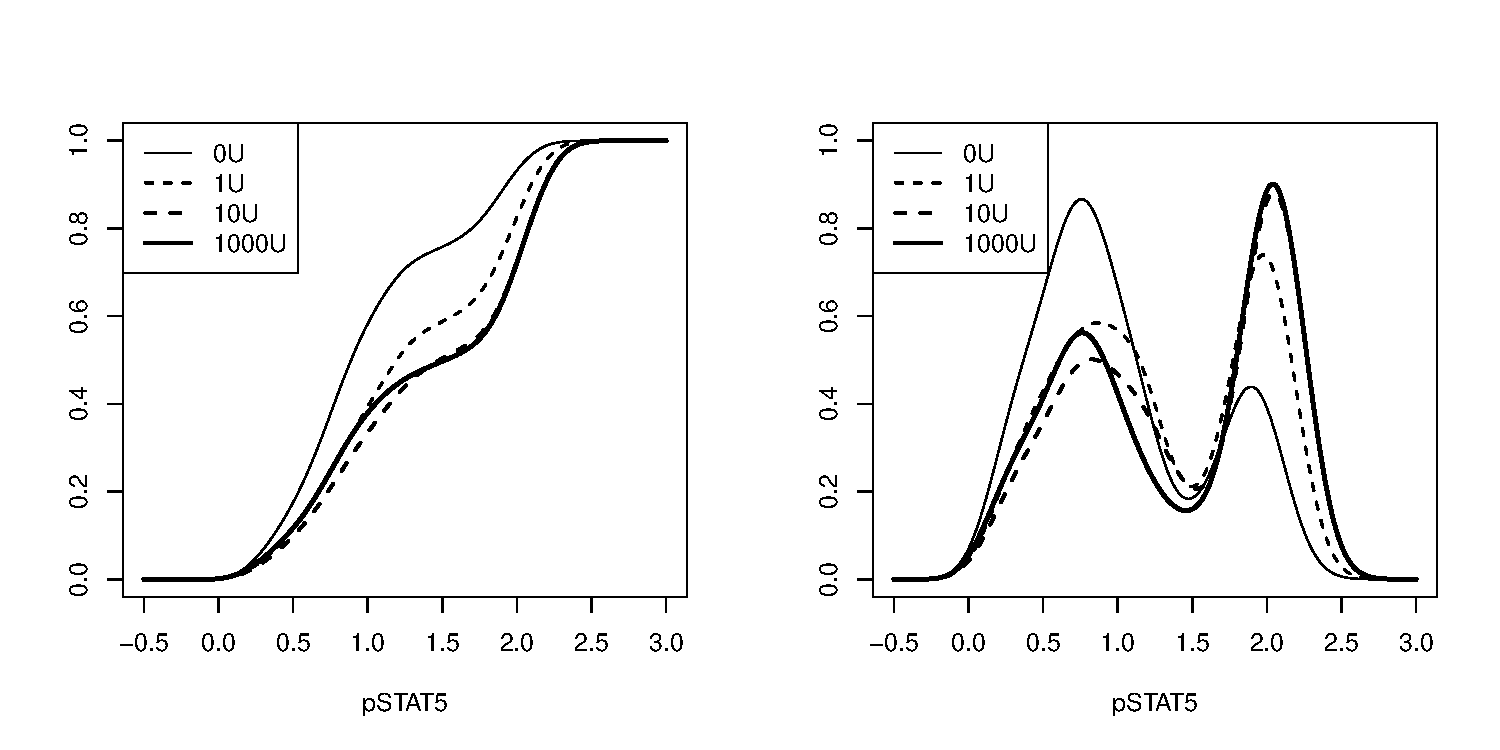
\includegraphics[scale=.5]{figures/ungated-dose-effect.pdf}
    %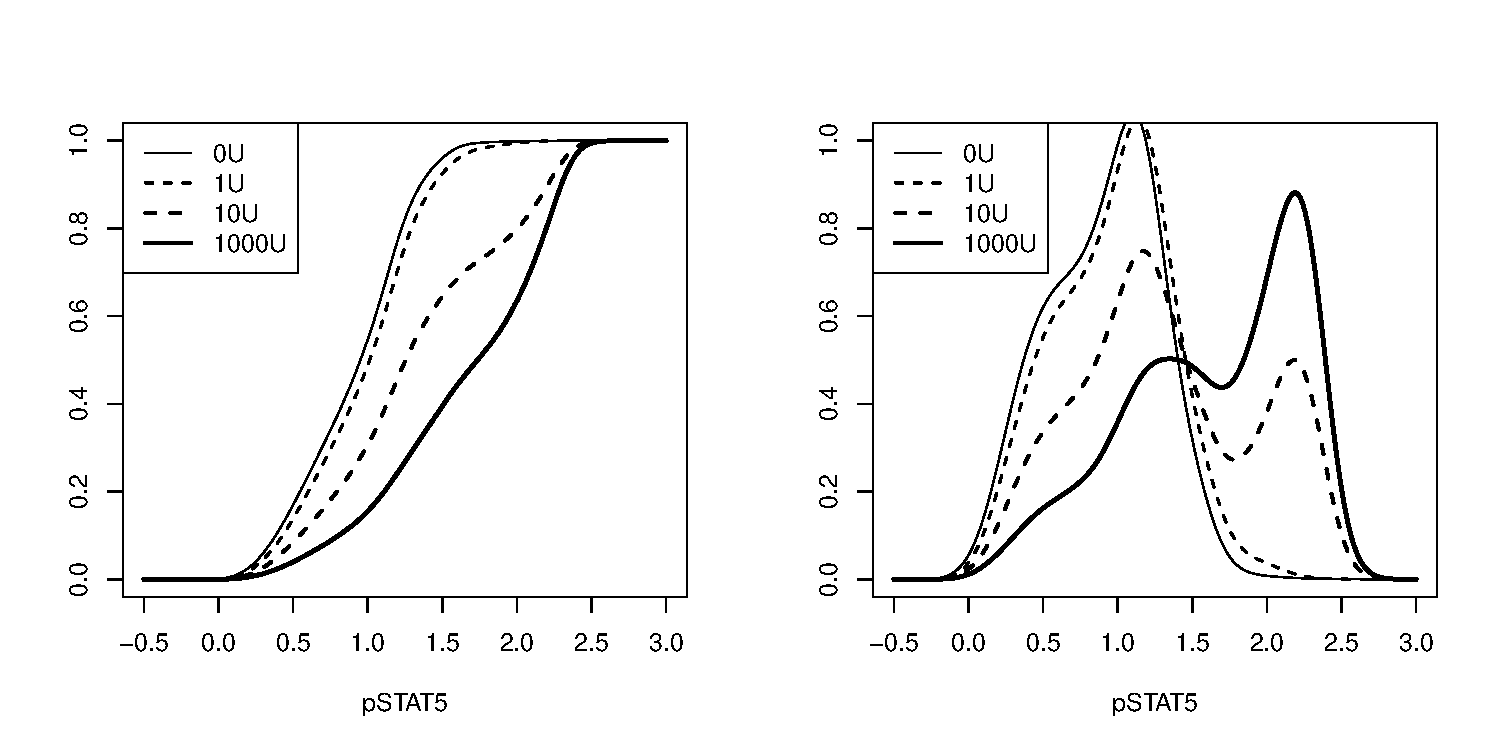
\includegraphics[scale=.5]{figures/lymph-dose-effect.pdf}
    %\mycaption{figure:dose-effect}
    %{Dose effect.}
    %{
        %On the left the cumulative density function obtained from individual a on day 1 across 4 increasing doses.
        %On the right the density function.
        %The top two figures are from the ungated sample.
        %The bottom two figures are from a CD4 range gate.
        %We observe that in the unstimulated sample the distribution is already bimodal 
        %and that upon stimulation the location of the peaks does not change much but that the height changes greatly.
        %Contrary to the ungated data, the pSTAT5 distribution in the CD4 gated sample now appears unimodal when resting or stimulated
        %at the lowest 1 units dose.  At the higher doses we start seeing a bimodal distribution.
        %In the ungated sample, the location of the activation peak seems to align somewhat with that of the activation peak.  }
%\end{figure}
%
%In \Cref{figure:dose-effect} we observe that at the lowest 0.1 units dose there seems to be a much more stronger relative repsonse
%in the whole sample than in the lymphocyte subset which suggests that there exist other cells beside CD4\positive lymphocytes
%which are also responsive to low doses of IL-2.  
%However the relative difference in response between 10 units and 1000 units seems much more important in lymphocytes than in the whole sample
%suggesting that the non-CD4\positive lymphocytes in the whole sample reach saturation at 0.1 units.
%Also since the resting sample sample displays a shoulder this suggests a mixture of resting and already semi-activated lymphocytes.

Using the normalisation methods described in the previous section, I was unable to significantly improve the reproducibility of this assay.
My view is that this dataset, as it stands, is not sufficiently reproducible to rigorously assess whether there is a difference in proleukin response between cases and controls in the cell subsets under study.
%Although our dataset is not amenable to this type of statistical analysis because of batch variation which is very difficult to correct
However, it may still contain useful biological information.
As described in \Cref{table:IL2-panels}, a subset of samples stained with a quite comprehensive panel, including CD3, CD56 and CD8, we can be used to address another clinically relevant question:
beside the four manually gated cell subsets, are there other subsets which respond to proleukin within the \gls{PBMC}?

This question is extremely relevant for DILT1D\footnote{\url{http://www.clinical-trials-type1-diabetes.com}} and other clinical trials of IL-2 which have mostly focused on lymphocytes.  %CD4\positive cells.
Biologists know that any cell which carries high levels of any of the trimeric components of the IL-2 receptor,
alpha (\protein{CD25}), beta (\protein{CD122}) or gamma (\protein{CD132}), should respond to IL-2,
but due to low affinity of the CD122 antibody and the limitation on the possible number of fluorochromes per tube, these cannot all be included as part of every flow experiment.  
%Plus at low doses of IL-2 the CD25 chain is the most important
%Also the gamma chain is expressed by all cells and so not specific
This study of \emph{ex vivo} stimulated whole blood offers the opportunity to identify other, potentially new, cell subsets also responsive to IL-2.
In order to increase my chances of characterising these subsets, I only analysed samples stained with the most comprehensive marker panel we had available, the one containing the additional fluorochromes for CD3, CD8 and CD56 (\Cref{table:IL2-panels}).
Unfortunately, the staining using this panel was of poor quality in many samples, due to the harsh nature of the permeabilisation protocol and to the larger number of markers used, which caused certain marker stains, such as CD56, to not work well across all batches.
%Furthermore, in the FCS files some channels were labelled by  a fluorochrome which was not in fact included in the sample.
This made between-batch analysis infeasible so instead, I focused on the analysis of a single batch for which the staining had worked. %within-batch analysis.
Assessing the staining quality of a sample requires prior knowledge, and so \contributor{Marcin Pekalski}, an experienced
flow cytometrist, assisted me in finding a batch with no obvious staining artefacts (\Cref{figure:tony-cd4-gating2} and \Cref{figure:lymphocytes-all-markers}).
This batch was then used for subsequent analysis in the rest of this chapter.
%which is only available in a subset of samples.
%Given the markers used in this study, I was interested in finding out if I could identify other cell subsets which are sensitive to proleukin.
%We are interested in identifying and classifying cell subsets by their sensitivity to proleukin.  

When assessing the dose-response to stimulation in a flow cytometry sample, the classic approach is to first gate cell populations in each sample based on their core markers,
then to assess the response of the functional marker in the gated subset.
Obviously, this approach is not exhaustive and consequently may miss other dose-responsive cell populations which are not included in the gating strategy.
Here I first explored approaches to visualise the pSTAT5 dose-response in the whole sample in order to spot other potential dose-responsive cell subsets.
I also considered more automated methods which use the pSTAT5 response to guide the identification of these cell subsets.
One of the challenges faced in identifying new cell types is how to reconcile the two different kinds of flow cytometric data, scatter and fluorescence, since these represent quite different physical properties and are measured on a linear and logarithmic scale respectively.
Typically scatter gating takes precedence over fluorescence gating, and the standard protocol is to first use scatter to discriminate live cells from debris.
In the next section, I followed this protocol, by first gating on side and forward scatter in order to distinguish lymphocytes from non-lymphocytes, then conducting separate analysis on the lymphocyte subset using fluorescent markers only, and to the non-lymphocyte subset, using both fluorescent and scatter markers.
%While the manual gating inspired approach is the established method, it suffers from a major drawback:
%it relies on prior knowledge of the number of cell populations and consequently misses the pSTAT5 response in uncharacterised cell subsets.


\subsection{SPADE: spanning-tree progression analysis of density-normalized events}

Visualisation is a fundamental tool for exploring high dimensional datasets.
In this instance, I am interested in visualising the pSTAT5 response in the whole sample as a function of proleukin dose and a total of nine core markers, seven fluorescent markers and two scatter markers.
Dimensionality reduction methods can provide a two-dimensional representation of a higher dimensional data set from a distance matrix.
These methods are particularly suited for datasets with less data points but more dimensions than in flow cytometry,
as generated by mass cytometry technologies such as CyTOF.
In mass cytometry datasets, more emphasis is given on uncovering cell lineages and progressions rather than discrete cell populations which share marker
properties.
%\Gls{MDS} methods can give us an two-dimensional representation of a higher dimensional data set from a distance matrix.
Most of these methods, like \gls{MDS}, require computation of the complete pairwise distance matrix,
but some like \gls{PCA} can use the covariance matrix instead to identify the components which accounts for most of the variation. 
%There are well established linear ones such as \gls{PCA} but also nonlinear ones such as \gls{ISOMAP} \citep{Tenenbaum:2000jp}.
%Stochastic neighbour embedding attempts to preserve the proximity of objects in higher dimensional space by using probabilistic mapping of higher dimension space to lower dimension.
%A drawback is that the mapping is impossible to retrieve, which is why component methods like PCA and ICA are more interpretable.  
However, the structure in the data may be poorly represented by the principal components since certain cell populations are unlikely to be linearly separable.
Therefore, there is considerable interest in developing methods that capture both the local and global structure of the data, so that points which lie close in higher-dimensional space tend to lie close in two-dimensional space.
%\gls{ISOMAP} \citep{Tenenbaum:2000jp}.
%SPADE is a methods which was developed with this objective.
In flow cytometry, one such method is \acrfull{SPADE} which yields a \acrfull{MST} representation,
where each node in the tree represent a multi-dimensional cluster in flow marker space \citep{Simonds:2011jh}.
The \gls{MST} is defined as the shortest path that connects all points in a network.
%The visualisation requires requires downsampling.
%A soft approach to downsampling, is to downweight points in high-density regions
The computation of the \gls{MST} requires the distance of every point to every other point to be known, hence the complete distance matrix must calculated.
However, it is too large to fit in computer memory for most ungated flow cytometry samples which can contain millions of data points.
%since the number of data points far exceeds.
Hence \gls{SPADE} first needs to reduce the number of data points by making use of downsampling and clustering.
In order for all existing regions of the marker space to be equally represented in the reduced dataset, the density is normalised across the sample.

\hspace{-2cm}
\begin{figure}[h]
\centering
%\includegraphics[scale=.5]{figures/manual-gating.pdf}
\begin{subfigure}[c]{.45\linewidth}
    \centering
  \includegraphics[scale=.65]{figures/downsampling-200.pdf}
\caption{Downsample 200}
\end{subfigure}
\begin{subfigure}[c]{.45\linewidth}
    \centering
  \includegraphics[scale=.65]{figures/downsampling-50.pdf}
  \caption{Downsample 50}
\end{subfigure}
\mycaption{figure:downsample}{ Example of density-dependent downsampling on bivariate 50,0000 point dataset on CD45RA and CD25. }
{
Effect of density-dependent downsampling from 50,000 to 200 datapoints (a), and density-dependent downsampling to 50 datapoints (b). 
The size of the green points represent the density.
The small top-right cloud of points is preserved after density dependent down-sampling.
}
\end{figure}

At each data point, the multivariate density is estimated, then the number of points is reduced by preferentially removing 
points with high local density while preserving lower density ones (\Cref{figure:downsample}).
%Hence the density is more uniform across the sample.
%This is that the density has less influence on the clustering.
Once the number of points has been reduced to some target number or by some factor, in each individual sample,
the samples are pooled and agglomerative clustering is applied.
%further reducing the number of data points to set number .
%The overall number of clusters can then be selected by cutting the resulting dendogram at the required height.
%The default parameter is 300 clusters.
The distance matrix is then calculated on the clusters and they are joined as nodes by the \acrfull{MST} algorithm for the purpose of visualisation.
%Once the MST has been constructed,
The points from each sample which were discarded in the density normalisation step, are then added back and assigned to their closest node in the tree.
%Hence the size of each cluster is sample dependent.
Hence the structure of the tree is the same across all samples but the size of the tree nodes 
is dependent on the number of data points assigned to each node per sample.
The tree nodes can then be coloured according to the intensity of a functional marker, for example here pSTAT5,
which was not used in its construction.
Two steps of the algorithm require user specified parameters, the parameter that defines the downsampling,
which can either be a target number of data points of a factor, and parameter that defines the number of desired clusters
in the agglomerative clustering step.

\paragraph{Lymphocytes}

I first ran \gls{SPADE} on the manually gated lymphocyte subset (excluding doublets),
in the resting and stimulated samples from an individual.
The algorithm was ran on the core surface markers, CD25, CD3, CD4, CD45RA, CD56, CD8 and FOXP3,
which are expected to be stable across within-batch stimulation doses.
The number of events in each sample was reduced by a factor of 90 percent.
The desired number of cluster in the agglomerative step was set to 1000.
The layout of the resulting \gls{MST} was determined by the \Rfunction{SPADE.layout.arch}
which aims to orientate the longest branch of an \gls{MST} along an arch with shorter offshoot branches hanging below.
The nodes in the tree were then coloured according to the fold increase in median pSTAT5 compared to the same node
in the resting sample (\Cref{figure:spade-lymphocytes-pstat5mfi}).
%The color scale was chosen to go from dark blue to red and the range was divided in percentiles.
%The output is presented in \Cref{figure:spade-lymphocytes-pstat5mfi}.
%In the unstimulated sample, th(\Cref{figure:spade-lymphocytes-pstat5mfi}a)
The initial pSTAT5 response to the lowest $0.1$ units dose proleukin, clusters in two regions of the tree,
as seen in \Cref{figure:spade-lymphocytes-pstat5mfi}b.
As the stimulation dose is increased to $10$ units, the level of the response increases in these two regions,
and there are signs of response in further adjacent nodes of the tree (\Cref{figure:spade-lymphocytes-pstat5mfi}c).
Finally at the highest dose of $1000$ units, the majority of the nodes show some level of response (\Cref{figure:spade-lymphocytes-pstat5mfi}d).

In order to discover where the responsive cells lie on the tree in relation to the cells identified using manual gates, I mapped the cells labelled by manual gating as memory and naive, both Teffs and Tregs, cells onto their assigned tree nodes (\Cref{figure:spade-lymphocytes-celltypes}a).
I found that the manually identified cell types tend to appear in neighbouring tree nodes with a few in other locations of the tree.
Also, memory Teffs and Tregs lie closer to each other than naive Teffs and Tregs (\Cref{figure:spade-lymphocytes-celltypes}a).
From visual inspection, the pattern of pSTAT5 response in the \gls{MST} corresponds to the locations of the cell types
with the memory and naive Tregs showing the first signs of response at $0.1$ units, memory Teffs starting to show activation at $10$ units,
followed by naive Teffs at $1000$ units.

In \Cref{figure:spade-lymphocytes-celltypes}b, a number of dose-responsive tree nodes which lie far on the main branch from the other studied subsets, were selected and the cells they contain were projected back to marker space.
Thus, I could visualise where these cells lay in relation to the known subsets (\Cref{figure:spade-lymphocytes-clusters}).
These cells constitute approximately one percent of the cells in the lymphocyte subset.
As depicted in \Cref{figure:spade-lymphocytes-clusters}, some properties of these cells distinguishes them from naive and memory subsets.
They are CD56\high, CD3\negative, CD4\negative, CD8\positive and express moderate levels of CD25.
%These cells could include CD56 bright cells,
%a cell subset currently under investigation by \contributor{Charlie Bell} using RNAseq,
%which are known to express high levels of CD122 (the beta chain of the IL2 receptor),
%but they are CD3\positive whereas those cells are CD3\negative.
Since those cells are CD8\positive CD56\positive they are probably \gls{NK} like cells, and may have cytotoxic properties.
These cells constitute $1.14$ percent of all lymphocytes.
However they are only stimulated somewhere between 10 and 1000 units of proleukin so may not be influential at the low doses used in DILT1D.

\begin{figure}[h!]
\centering
\begin{minipage}{.7\textwidth}
\includegraphics[width=\linewidth]{figures/spade-lymphocytes-pstat5mfi}
\end{minipage}
\mycaption{figure:spade-lymphocytes-pstat5mfi}
{Lymphocytes: \gls{MST} generated by applying \gls{SPADE} on lymphocytes. \gls{MST} nodes are coloured by pSTAT5 \gls{MFI}.}
{
  The \gls{MST} was constructed from running \gls{SPADE} on the core surface markers,
  CD25, CD3, CD4, CD45RA, CD56, CD8 and FOXP3, in the manually gated lymphocyte subset (after double exclusion),
  pooled across the four stimulation doses in a sample from one individual.
  The required number of clusters in the agglomerative clustering step was set to k=1000.
  %The size of each node in the tree is representative of the number of cells which are assigned to that cluster. 
  The colouring of the nodes from dark blue to bright red follows the pSTAT5 MFI fold increase.
  In samples where the proleukin dose is increased, more nodes in the tree are illuminated since the pSTAT5 MFI increases in various cell subsets.
  The size of the tree nodes are proportional to the number of cells in the data file which are assigned to that node.
}
\end{figure}

\begin{figure}
\centering
\begin{minipage}{\textwidth}
\includegraphics[width=\linewidth]{figures/spade-lymphocytes-celltypes}
\end{minipage}
\mycaption{figure:spade-lymphocytes-celltypes}
{ Lymphocytes: (a) Mapping of cell types defined by manual gates onto the \gls{MST} obtained in \Cref{figure:spade-lymphocytes-pstat5mfi}.  (b) Manually identified subset of cells, \texttt{SPADE.1} (purple), which respond to 1000 units but lie far from the other manually gated cell subsets. }
{ (a)
The different manually gated cell types do not always segregate to different branches but can be spread across the tree.
For example, naive Teffs appear in different regions of the tree.
Furthermore, certain nodes of the tree can contain a mixture of cell types which complicates the interpretation.
In order to guard against this, the number of clusters in the agglomerative clustering needs to be set to a high number.
(b)
Manual identification of a 1000 units responsive subset of cells (blue line) which lies far from the manually gated cell populations.
The \gls{MST} was generated on the lymphocytes stimulated at 1000 units and coloured by the pSTAT5 MFI fold increase.
}
\end{figure}

%
\begin{figure}
\centering
\begin{minipage}{.65\textwidth}
\includegraphics[width=\linewidth]{figures/spade-lymphocytes-clusters}
\end{minipage}
\mycaption{figure:spade-lymphocytes-clusters}
{ Lymphocytes core markers: A 1000 unit responsive cell subset \texttt{SPADE.1} within lymphocytes is identified which is not assigned to any manual gate.  }
{ The subset of cells, delineated in purple, manually identified in \Cref{figure:spade-lymphocytes-celltypes}, is distinct from the manually gated cell subsets memory Teffs, memory Tregs, naive Teffs and naive Tregs. Its discriminating features are that it is CD4\negative, high for CD8 and CD56, while expressing moderate levels of CD25.
} 
%
\begin{minipage}{.5\textwidth}
  \includegraphics[scale=0.4]{figures/spade-lymphocytes-dose-response}
\end{minipage}
\begin{minipage}{.3\textwidth}
\mycaption{figure:spade-lymphocytes-dose-response}
{ Lymphocytes pSTAT5 MFI dose-response: Newly identified cell subsets within lymphocytes. }
{
In purple, the newly identified cell subsets \texttt{SPADE.1} in \Cref{figure:spade-lymphocytes-celltypes} only shows response at 1000 units of proleukin. 
}
\end{minipage}
\end{figure}

\clearpage

\paragraph{Non-lymphocytes}

In order to see whether I could detect other cell subsets besides lymphocytes, which respond to proleukin,
I reran \gls{SPADE} on the same dataset, this time excluding cells lying within the lymphocyte scatter gate,
but including forward and side scatter as markers in the clustering.
While at 0.1 units little response was seen (\Cref{figure:spade-nonlymphocytes-pstat5mfi}b), two small clusters showed response at 10 units, highlighted in blue and purple, and at 1000 units, a much larger cluster highlighted in pink (\Cref{figure:spade-nonlymphocytes-pstat5mfi}c and d).

\myfigure{scale=.65}{spade-nonlymphocytes-pstat5mfi}
{Non-lymphocytes: pSTAT5 MFI coloured \gls{MST} generated by applying \gls{SPADE} on cells which fall outside of the lymphocyte gate.}
{
  Three subsets of cells are manually identified which show response to proleukin at 10 units (highlighted in blue and purple on d),
  and 1000 units (pink).
  %The \gls{MST} was constructed from running \gls{SPADE} on the core surface markers,
  %CD25, CD3, CD4, CD45RA, CD56, CD8 and FOXP3, in cell which do not belong to the lymphocyte gate, of four samples from one individual,
  %stimulated at increasing doses of proleukin.
  %As the proleukin dose is increased more clusters in the tree are illuminated, as the pSTAT5 MFI increases in various cell subsets.
  %The size of each node in the tree is representative of the number of cells which are assigned to that cluster. 
  %No nodes in the tree appear to be brightly illuminated which suggests that the pSTAT5 response is low or not detectable using SPADE.
}
% 

I manually selected these groups of nodes and projected them back to forward and side scatter space to see where they lay in relation
to the lymphocyte cluster (\Cref{figure:spade-nonlymphocytes-scatter-clusters}).  
%One observation is that these cells do not seem to cluster well on side and forward scatter.
I found that these three groups (blue, purple and pink) cluster around the lymphocyte scatter gate which suggested that there are no detectable clusters of cells which fall within the other major scatter clusters which constitute physically larger and more granular cells such as monocytes
or granulocytes (\Cref{figure:spade-nonlymphocytes-scatter-clusters}).
The cells responsive to the lower 10 unit dose of proleukin (in light blue and purple) cluster closer to the lymphocyte scatter
(\Cref{figure:spade-nonlymphocytes-scatter-clusters}a)
than the large 1000 unit responsive subset of cells (in pink) (\Cref{figure:spade-nonlymphocytes-scatter-clusters}b),
suggesting that the former are more likely to be lymphocytes which were not included in the manual gate.
While the larger population (pink) also tends to aggregate around the lymphocyte scatter it
further appears to aggregate in another potential, less well defined, scatter cluster, delineated by the purple polygon in \Cref{figure:spade-nonlymphocytes-scatter-clusters}b.

\myfigure{scale=.5}{spade-nonlymphocytes-scatter-clusters}
{
    Non-lymphocytes: \texttt{SPADE.1}, \texttt{SPADE.2} and \texttt{SPADE.3} mapped back to forward and side scatter coordinates.
}
{
    The three cell subsets, blue, purple and pink, manually identified in the \gls{MST} of \Cref{figure:spade-nonlymphocytes-pstat5mfi}  are mapped back to scatter coordinates.
  The 10 unit responsive groups, blue and purple points in (a), and the 1000 units responsive group, pink points in (b),
  generally tend to lie close to the lymphocyte cluster (black ellipse), but a potential secondary scatter cluster of 1000 unit responsive cells
  (delineated by the purple polygon) are worthy of further investigation.
  %The cell subsets manually identified in \Cref{figure:spade-nonlymphocytes-pstat5mfi} as responding to 10 units of proleukin (blue and purple) in (a)
  %and 1000 units of proleukin (pink) in (b), are mapped back to the forward and side scatter channel.
  In order to visualise where the points lie in relation to the rest of the sample they are are overlayed on top of a sample in which lymphocytes are present.
  %While the 10 unit responsive cells cluster mostly around the lymphocyte gate, the 1000 unit responsive cells also appear to cluster within a secondary scatter cluster (purple polygon).
}

Following further investigation of this subset of cells on other core markers in \Cref{figure:spade-nonlymphocytes-clusters},
and after filtering of doublets on side scatter width and height,
while they appeared mostly CD3\positive, CD4\positive and CD56\negative therefore likely to be T cells or NKT cells,
they also contained a small fraction of CD3\negative cells,
hence likely to be a heterogeneous subset that may contain some monocytes.

%They contain both CD8\negative and CD8\positive cells.
As they are bigger on forward and side scatter than lymphocytes,
they could be bigger T cell blasts, and as they are mostly CD45RA\positive,
possibly activated T cells.
%what about CD56?
However, they may well result from a technical artefact of the fixation protocol.
Further markers, possibly monoycte markers such as CD19, are needed to better define this cell type
and ascertain its clinical relevance.



\begin{figure}
  \centering
\begin{minipage}{.9\textwidth}
\includegraphics[width=\linewidth]{figures/spade-nonlymphocytes-clusters}
\mycaption{figure:spade-nonlymphocytes-clusters}
{ Non-lymphocytes: \texttt{SPADE.1} subset of cells in relation to lymphocyte cluster on all markers.  }
{ After filtering of doublets on the the side scatter height, the \texttt{SPADE.1} cluster defined on side and forward scatter in \Cref{figure:spade-nonlymphocytes-scatter-clusters} is displayed on the other core markers.  The cluster appears to be quite heterogeneous but contains predominantly CD3\positive, CD4\positive, CD45\positive and high for CD25.  } 
\end{minipage}
%
\begin{minipage}{.5\textwidth}
  \includegraphics[width=\linewidth]{figures/spade-nonlymphocytes-dose-response}
\end{minipage}
\begin{minipage}{.3\textwidth}
\mycaption{figure:spade-nonlymphocytes-dose-response}
{ Non-lymphocytes: Dose-response }
{ The gray line represents the whole sample.  The black line is the lymphocyte population and the purple line is the \texttt{SPADE.1} subset identified in \Cref{figure:spade-nonlymphocytes-scatter-clusters}.  }
\end{minipage}
\end{figure}


\clearpage



%\paragraph{Pooling}
%
%SPADE requires pooling samples for identification of the clusters which are later used in the construction of the \gls{MST}.
%which is not advisable given that the core markers are not stable in ungated data across batches because of debris.
%
%However the underlying agglomerative clustering which is used to build the MST, gives good coverage of the whole markers space.
%This allows the pSTAT5 distribution to be assessed per cluster.
%However because of the downsampling step, this introduces some stochasticity in the clustering which can lead to different results
%on the same dataset depending on which points are dropped.
%Furthermore the multivariate density estimation step can also include randomness if approximate schemes are used to improve performance.
%These 
%
%Since the clusters are defined by pooling all downsampled tubes, and then upsampling them per tube,
%their sizes tends to change depending on the tube.
%Clusters whose proportion changes significantly between tubes are likely to be debris.
%The other criterion to consider is the fold change of the pSTAT5 MFI in each cluster.
%a feature of SPADE which proves useful is the downsampling and agglomerative clustering which aims to identify lower density clusters.
%The pSTAT5 distribution can be assessed in each of these clusters.
%
%If pSTAT5 were to be included the clustering, then the size of the nodes would reflect the change in pSTAT5 activation and so it would be
%difficult to distinguish whether the noise of the pSTAT5 influences more the size of the node.
%
%
%%\paragraph{The influence of scatter on spade}
%If left untransformed, the forward and side scatter bare a lot of influence on the clustering since they typically very large ranges.
%Furthermore, scatter is not amenable to logarithmic scaling since, unlike fluorescence, it does not scale multiplicatively.
%To remedy this I considered the following two options, either first cluster on the side and forward scatter using mixture models
%and then run spade on each scatter cluster individually,
%or, scale the scatter so that it appears on a similar scale as the fluorescence.
%%It is also unclear to me whether scatter should feature in the density estimation and clustering.
%%This is a general problem when trying to include variables of a very different nature.
%%In cell biology is size more important than surface marker intensity?
%%The challenge is that on one hand we have a covariate that scale multiplicatively (fluorescence) and on the other
%%we have a covariate that scales linearly.
%An advantage of the first approach is that it removes many spurious events which are likely to be noise and so more spade clusters are
%dedicated to relevant events.
%%scatter clusters can be examined in closer detail.
%The disadvantage is that certain of the events which are filtered based on scatter may be biologically relevant.
%Hence I tried and compared the output of both approaches.
%
%%\myfigure{scale=.75}{scatter-gating4}
%%{ }
%%{ }
%

\subsection{\label{RPART} RPART: recursive partitioning on core markers} 

The \gls{SPADE} approach first clustered on the core markers across batches,
%four aliquots of the same sample stimulated at different concentrations of proleukin,
then built the \gls{MST} from these, allowing for visual identification of
clusters with a high pSTAT5 response.
The clustering was preceded by a downsampling step which aimed to make the density
more uniform across the sample so that all points had an equal probability of being
represented as part of a distinct cluster.  
%SPADE used clusters defined from running agglomerative clustering on pooled downsampled datasets.
%In the upsampling step of the algorithm when points are assigned to their closest cluster, they influence the size of the cluster but also update their median.
%While this should not be the case provided the core markers are stable, if this not the case then the location of the clusters will be different depending on the sample.
An alternative to clustering across samples, is to use recursive partitioning instead to split the core marker space into bins containing roughly the same number of
events across samples within the same batch.
%A partition one sample on the the core marker
%space into bins containing approximately the same number of events,
%then the same partitioning scheme across samples within the same batch.
This can be achieved by recursively splitting on the median of each marker, so that at each split, half of the dataset is assigned to each of the two branches.
The process is applied recursively to each bin until a minimum bin size or maximum number of recursive steps is reached.  
Typically, the order in which the markers are selected is guided by picking the marker
with the largest variance or range at each split.
Since each bin contains approximately the same proportion of events,
this implies that the binning is finer in regions of high density and coarser in regions of low density.
Provided that the number of bins is sufficiently large, this is conceptually another approach of reducing the number of events while preserving lower density regions, similar to the method of density-dependent downsampling.
%but instead of thinning the data, the bin size changes
Recursive partitioning was first introduced to flow cytometry by \citet{Roederer:2001tz},
under the name of ``probability binning'', as a means of translating a multivariate distribution into a univariate one,
in order to test statistical significant differences in event counts between individual bins or whole samples.
The algorithm was later implemented in the \BioConductor{flowFP} as ``flow cytometric fingerprinting'' and has been
applied to discriminate bins which differ significantly in proportion between healthy controls and \gls{AML} patients
\citep{Rogers:2008ij,Rogers:2009jz}.
% first came prob binning, then frequency difference gating and lastly fingerprinting
%The approach was later extended to multiple dimensions with the ``flow cytometric fingerprinting'' method as implemented in
%the \BioConductor{flowFP},
%by using multidimensional bins.% .
%it also used by kd trees
%in the form of frequency difference gating,
%a binary space partitioning technique in which data is iteratively partitioned along the median.
%flowBin
%Software to combine flow cytometry data that has been multiplexed into multiple tubes with common markers between them, by establishing common bins across tubes in terms of the common markers, then determining expression within each tube for each bin in terms of the tube-specific markers.
%The \BioConductor{flowBin} package uses this process to join samples on common markers across tubes and then to determine the expression within each bin of tube specific markers.
%Binning can be used to identify regions where the proportion of events changes significantly between samples
%or as a measure to determine the distance between two flow cytometry samples.
%However, the binning process is obviously sensitive to noise so methods which are point centric rather than based on regions are preferred.
%All these approaches are based on the idea of recursive partitioning of a high dimensional space to reduce the dimensionality of the dataset.
%These are ideas I explore next with \acrfull{CART}.


%\paragraph{Binary recursive partitioning on core markers} 
%Roederer, M., Moore, W., Treister, A., Hardy, R. R., & Herzenberg, L. A. (2001). Probability binning comparison: a metric for quantitating multivariate distribution differences. Cytometry Part A, 45(1), 47–55. doi:10.1002/1097-0320(20010901)45:1<47::AID-CYTO1143>3.0.CO;2-A
For the purpose of visualisation, I first illustrate the recursive partitioning algorithm on side and forward scatter using 128 bins (\Cref{figure:scatter-rpart-128bin-var}).
The binning was defined by pooling all four samples on side and forward scatter.
Since each bin should contain approximately $\dfrac{1}{128^{th}}$ of the events, finer binning is applied to higher density regions and coarser binning to sparser regions.

\begin{figure}[!h]
    \centering
    \includegraphics[scale=.75]{figures/scatter-rpart-128bin-var}
\mycaption{figure:scatter-rpart-128bin-var}
{Sample recursively partitioned into 128 bins on side and forward scatter.}
{
   The binning is determined in the resting sample (a) and then the same binning is applied across all samples (b, c and d).
   While each each bin contains the same number of events in the resting sample (a), this does not necessarily hold in the
   other samples (b, c and d).
}
\end{figure}

Applying the same binning across the four samples, the relative proportion of events assigned to each bin varies between samples (\Cref{figure:scatter-rpart-128bin-var-prop}).
%This is a potential shortcoming of the binning method, namely finding a binning scheme which minimises the between
If the number of bins is increased each bin represents a smaller proportion of the sample so consequently the variations between samples should also become smaller.
%In particular, bins highlighted in red in samples b, c and d of \Cref{figure:scatter-rpart-128bin-var-prop}
%coincide with high side scatter, low forward scatter, events which are only present in the unstimulated sample
%\Cref{figure:scatter-rpart-128bin-var}.  These events are likely to represent debris.
%and more generally when comparing distributions,

\begin{figure}
 \centering
\begin{minipage}{.65\textwidth}
 \includegraphics[width=\linewidth]{figures/scatter-rpart-128bin-var-prop}
\end{minipage}
\begin{minipage}{.3\textwidth}
\mycaption{figure:scatter-rpart-128bin-var-prop}
{Each sample is recursively partitioned using 128 bins.}
{
  The colour indicates whether the proportion of events increases (green) or decreases (red) relative to the mean in each bin across all samples.
}
\end{minipage}
\end{figure}

%
\begin{figure}
 \centering
\begin{minipage}{.65\textwidth}
\includegraphics[width=\linewidth]{figures/scatter-rpart-128bin-var-pstat5}
\end{minipage}
\begin{minipage}{.3\textwidth}
\mycaption{figure:scatter-rpart-128bin-var-pstat5}
{pSTAT5 response in sample recursively partitioned into 128 bins on side and forward scatter.}
{
    %The bins which first show  pSTAT5 response (b) are likely to be due to debris found in the resting sample (a)
    %but not in the stimulated samples (b, c and d).
  No pSTAT5 response is visible in any of the bins at 0.1 (b) or 10 (c) units.
  However at 1000 units (d), the bins which overlap with the location of the lymphocytes on side and foward scatter show strong response.
  Also the bin which coincides with the location of the cluster in \Cref{figure:spade-nonlymphocytes-scatter-clusters} shows some moderate response
  confirming that there is likely to be some responsive cells lying within that cluster.
}
\end{minipage}
\end{figure}

%Binning provides a convenient approach for standardising the number of events across samples.
The pSTAT5 response on side and forward scatter is visualised in \Cref{figure:scatter-rpart-128bin-var-pstat5} by colouring each bin by its median pSTAT5 response.
No pSTAT5 is visible in any of the 128 bins at 0.1 or 10 units (\Cref{figure:scatter-rpart-128bin-var-pstat5}b and c) which suggest that the proportion of
0.1 unit and 10 unit responsive cells is too small within each bin to influence the pSTAT5 median.
However at 1000 units, bins which overlap with the lymphocyte cluster show clear response as well as the bin which overlaps with the uncharacterised cells
delineated in pink in \Cref{figure:spade-nonlymphocytes-scatter-clusters}b.
%While three bins start to show response at 0.1 units (\Cref{figure:scatter-rpart-128bin-var-pstat5}b), they correspond to regions where the number proportion of events
%is much lower than in the resting sample (b, c and d of \Cref{figure:scatter-rpart-128bin-var-prop}).
%No response is visible in any other bins at 0.1 and 10 units \Cref{figure:scatter-rpart-128bin-var-prop}).
%Instead a more informative means of visualising potentially interesting bins is to plot
%bin properties such as the pSTAT5 response in each bin against the total change in proportion for each bin across samples
%(\Cref{figure:rpart-1024bin-var}).
%This provides a visual means of identifying bins which may show a large pSTAT5 response simply
%because of larger changes in the underlying proportion of events between samples as were identified
%in \Cref{figure:scatter-rpart-128bin-var-prop}.
%In \Cref{figure:rpart-1024bin-var}, I have highlighted potentially interesting bins which show small changes in proportion across samples
%but large increase in pSTAT5 response.  Projecting these bins back onto side and forward, these bins include the lymphocytes but also
%cover a larger area which includes cells outside of the lymphocyte cluster with a lower forward scatter (\Cref{figure:rpart-1024bin-var})b.
%\myfigure{scale=.65}{rpart-1024bin-var}
%{ pSTAT5 fold change between resting and 1000 units against change in proportion for recursive partitioning on all core markers (SSCA, FSCA, CD4, CD3, ) using 1024 bins. }
%{ The bins show the less change in proportion and the highest pSTAT5 response are highlighted in red (a) and plotted on side and forward scatter (b). }

%Discussion
%Since the order in which the markers are selected can vary between samples, the partitioning can differ significantly.
%This is the case if the distributions are significanlty different but may also be due to outliers inflating the variance across different samples.
%It may be worth first limiting the influence of outliers on the variance by first bounding the distributions
%or downweighting them by their influence.
%The other issue is that the mean and hence the variance is not representative of a multimodal distribution.
%Preserving the order of the splits while allowing for the bin locations to change complicates means that the bins
%may add too much variation.
%

\clearpage

\paragraph{Lymphocytes} 
Extending recursive partitioning to all core markers, I aimed to identify dose-responsive cells not assigned to any manual gate within the lymphocyte subset.
The number of bins was increased to 1024 and the recursive partitioning was ran on the core markers CD25, CD3, CD4, CD45RA, CD56, CD8 and FOXP3, on the lymphocyte subset, after excluding doublets.
I also excluded cells which were assigned to the manually gated subsets, both memory and naive, Teffs and Tregs, in order to focus on potentially unidentified cell subsets.
%%the size of the bins should be bigger though since points are sparser as we add dimensions
Since for any two dimensional projection of the data, many bins overlap, I used the same \gls{MST} visualisation as described in the previous section, where each node this time represents the core marker median of one of the 1024 bins (\Cref{figure:rpart-lymphocytes-mst-1024bin}).
Using the MST visualistion, I was able to identify a cluster of cells which responded to 1000 units.
%At 10 units, pSTAT5 response can be already seen one of the extreme of the tree.
From the MST, I visually identified two responsive cell subsets, a 10 unit responsive one (in pink) and a 1000 unit responsive cluster (delineated in purple).
Selecting the tree nodes manually and projecting the corresponding bins back to marker space, I plotted these two cell subsets in relation to the
manually gated subsets, memory Teffs (black), memory Tregs (red), naive Teffs (green) and naive Tregs (blue) (\Cref{figure:rpart-lymphocytes-clusters}).
The cell subset \texttt{RPART.2} delineated in pink constitutes around $4$ percent of the lymphocytes.
This cell subset contains moderate levels of CD25 similar to a memory Teffs and is CD3\positive, CD4\positive, CD8\negative, CD45RA\negative and FOXP3\negative.
It is likely to represent the transitional cell population between memory Teffs and Tregs which was not included in the manual gating.
On the other hand, the cell subset \texttt{RPART.1} delineated in purple appeared to be CD3\negative, CD4\negative, CD8\negative and high for CD56.
These cells were also low in CD25, with the same level of expression as naive Teffs, explaining their limited response at lower doses.
They constitute around $1.66$ percent of the total lymphocyte population within this sample.
These CD56 bright cells include CD3\negative cells so could belong to a cell subset currently under investigation by \contributor{Charlie Bell} in our lab using RNAseq,
which are known to express high levels of CD122, the beta chain of the IL2 receptor.

\begin{figure}
\centering
\includegraphics[scale=.7]{figures/rpart-lymphocytes-mst-1024bin}
\mycaption{figure:rpart-lymphocytes-mst-1024bin}
{ Lymphoyctes: MST built using the 1024 bins obtained from recursive partitioning on the lymphocytes core markers.}
{ A cluster of cells delineated in purple, \texttt{RPART.1}, shows pSTAT5 response at 1000 units and lies in a different part of the \gls{MST} from the remainder of the dose-responsive cells.  }
\end{figure}

\begin{figure}
\centering
\begin{minipage}{.8\textwidth}
\includegraphics[width=\linewidth]{figures/rpart-lymphocytes-clusters}
\end{minipage}
\mycaption{figure:rpart-lymphocytes-clusters}
{  Lymphoyctes: A 10 unit responsive cell subset (pink) and a 1000 unit responsive cell subset (purple) within lymphocytes are identified which are not assigned to any manual gate.  }
{
  Two subset of cells, a 10 unit responsive subset delineated in pink and a 1000 unit responsive subset delineated in purple,
  manually identified in the MST of \Cref{figure:rpart-lymphocytes-mst-1024bin},
  which are distinct from the manually gated cell subsets memory Teffs (black), memory Tregs (red), naive Teffs (green) and naive Tregs (dark blue),
  are projectd back to core marker space.
  The pink cell subset overlaps with the manually identified cell subsets
  Its discriminating features are that it is CD3\negative, CD4\negative and high in CD56, while expressing low levels of CD25.
  %clusters in one of the branches which does not overlap with any of the manual gates as seen in \Cref{figure:spade-celltypes}b.
%Projecting these cells back to intensity space it surfaces that they are CD4\negative which explains why they were not included in the manual gating.
%They are also CD45RA\negative and high for CD25 which explains why they respond to proleukin.
}
%\end{figure}
%
%\begin{figure}
    %\centering
\begin{minipage}{.5\textwidth}
    %\includegraphics[width=\linewidth]{figures/rpart-lymphocytes-dose-response}
  \includegraphics[scale=.4]{figures/rpart-lymphocytes-dose-response}
\end{minipage}
\begin{minipage}{.3\textwidth}
\mycaption{figure:rpart-lymphocytes-dose-response}
{  Lymphoyctes: Dose response of the cell subsets, \texttt{RPART.1} and \texttt{RPART.2}, within the lymphocytes in relation to the other cell subsets. }
{ }
\end{minipage}
\end{figure}

\clearpage


\paragraph{Non-lymphocytes}

Recursive partitioning was next applied to non-lymphocytes, in order to detect potentially new responsive subsets.
As side and forward scatter need to be included in the recursive partitioning of non-lymphocytes,
I scaled the scatter so as to have a similar range to the fluorescent markers.
%which were transformed using the previously described \Rfunction{logicleTransform}.
I again used 1024 bins although this number could have been increased because we are dealing with larger number of cell.
The recursive partitioning was run on the same markers but this time also included the side and forward scatter.
Once more, the MST was used to visualise the response across the whole sample (\Cref{figure:rpart-nonlymphocytes-mst-1024bin}).
At 0.1 units, no clear response is visible (\Cref{figure:rpart-nonlymphocytes-mst-1024bin}b) but at 10 units
(\Cref{figure:rpart-nonlymphocytes-mst-1024bin}c) certain nodes show moderate response within a branch of the MST which
later become part of cluster (delineated in purple) which shows strong response at 1000 units (\Cref{figure:rpart-nonlymphocytes-mst-1024bin}d).
Projecting the cells contained within this cluster back to marker space (\Cref{figure:rpart-nonlymphocytes-scatter-clusters}), 
they seem to lie close to the lymphocyte cluster (black) on side and forward scatter and also appear to contain both CD4\negative and CD4\positive cells.
They also overlap on side and forward scatter with the cluster identified in \Cref{figure:spade-nonlymphocytes-scatter-clusters}.

\begin{figure}[!h]
\begin{minipage}{\textwidth}
\centering
\includegraphics[scale=.6]{figures/rpart-nonlymphocytes-mst-1024bin}
%\end{minipage}
%\begin{minipage}{.3\textwidth}
\mycaption{figure:rpart-nonlymphocytes-mst-1024bin}
{ Non-lymphocytes: MST built on the 1024 bins obtained from \texttt{RPART} on non-lymphocytes. }
{
    A cluster of cells, \texttt{RPART.1}, (purple) stands out that shows pSTAT5 response at 1000 units.
} 
\end{minipage}
%\end{figure}
%
%\begin{figure}
\begin{minipage}{.6\textwidth}
\includegraphics[scale=.5]{figures/rpart-nonlymphocytes-scatter-clusters}
\end{minipage}
\begin{minipage}{.3\textwidth}
\mycaption{figure:rpart-nonlymphocytes-scatter-clusters}
{ Non-lymphocytes:  A 1000 unit responsive cell subset (purple) is identified which does not belong to the lymphocytes population (black).  }
{
In order to visualise where the points lie in relation to the rest of the sample they are are overlaid on top of a sample in which lymphocytes are present.
The subset of cells, delineated in purple, was manually identified in \Cref{figure:rpart-nonlymphocytes-mst-1024bin}.
}
\end{minipage}
\end{figure}

\begin{figure}
  \centering
\begin{minipage}{.9\textwidth}
\includegraphics[width=\linewidth]{figures/rpart-nonlymphocytes-clusters}
\mycaption{figure:rpart-nonlymphocytes-clusters}
{ Non-lymphocytes: core markers. }
{
    A 1000 unit responsive cell subset, \texttt{RPART.1}, in purple, is identified which does not belong to the manually defined lymphocyte population, in black. 
  %It is very similar to lymphocytes except on side and forward scatter so could 
  %In order to visualise where the points lie in relation to the rest of the sample they are are overlayed on top of a sample in which lymphocytes are present.
  %The subset of cells, delineated in purple, was manually identified in \Cref{figure:rpart-nonlymphocytes-mst-1024bin}.
}
\end{minipage}
%
\begin{minipage}{.5\textwidth}
\includegraphics[width=\linewidth]{figures/rpart-nonlymphocytes-dose-response}
\end{minipage}
\begin{minipage}{.3\textwidth}
\mycaption{figure:rpart-nonlymphocytes-dose-response}
{ Non-lymphocytes: Dose-response. }
{
 A 1000 unit responsive cell subset (purple) is identified which does not belong to the manually defined lymphocytes population (black).
  %In order to visualise where the points lie in relation to the rest of the sample they are are overlayed on top of a sample in which lymphocytes are present.
  %The subset of cells, delineated in purple, was manually identified in \Cref{figure:rpart-nonlymphocytes-mst-1024bin}.
}
\end{minipage}
\end{figure}




\clearpage


\subsection{PLSR: partial least squares regression}

So far, the only visualisation I have explored is the \gls{MST}, a non-linear projection of a multivariate dataset.
However, no information about the pSTAT5 response is captured in the layout of the tree, instead, I used colour to visually identify clusters with increased pSTAT5 MFI response.
An alternative may be to include the pSTAT5 in the linear projection using a technique known as \acrfull{PLS}.
\gls{PLS} is based on the well established \gls{PCA} method which decomposes the covariance matrix into orthogonal linear combinations of the variables, know as principal components, where each principal component succcessively captures most of the residual variation in the sample.
However while in PCA all variables are treated the same, in PLS, variables can be specified as response variable Y or predictors X.
%\gls{PLS} tries to find the covariates which best explains the regression
The general underlying model of the multivariate \gls{PLS} is then:
\[
    \pmb{X} = \pmb{T} \pmb{P}^{\top} + \pmb{E}
\]
\[
    \pmb{Y} = \pmb{U} \pmb{Q}^{\top} + \pmb{F}
\]
where $\pmb{X}$ is an n $\times$ m matrix of predictors and \pmb{Y} is an n $\times$ p matrix of responses.
$\pmb{T}$ and $\pmb{U}$ are n $\times$ l orthogonal matrices that are, respectively, projections of $\pmb{X}$ and projections of $\pmb{Y}$.
The matrices $\pmb{P}$ and $\pmb{Q}$ are, respectively, m $\times$ l and p $\times$ l orthogonal loading matrices.
The matrices $\pmb{E}$ and $\pmb{F}$ are the error terms, assumed to be independent and identically distributed random normal variables.  
%X and Y are the score matrices, and T and U are the orthogonal loading matrices.
The decompositions of $\pmb{X}$ and $\pmb{Y}$ are made so as to maximise the covariance between $\pmb{T}$ and $\pmb{U}$.
%Essentially, this approach is like doing PCA on two independent datasets, X and Y, and then rotating the solutions for maximum correlation
%subject to the covariance between the orthogonal loading matrices, T and U, being maximised.

I applied partial least squares regression,
%fitted with the kernel algorithm
using the \Rfunction{plsr} implementation in the \Rpackage{pls}, to both the lymphocytes and non-lymphocytes.
%

\paragraph{Lymphocytes} 
\begin{figure}[!h]
\centering
\includegraphics[scale=.7]{figures/plsr-lymphocytes}
\mycaption{figure:plsr-lymphocytes}
{ Lymphocytes: First two components of \gls{PLS} projection using pSTAT5 as response.}
{
Three new clusters, \texttt{PLSR.1}, \texttt{PLSR.2} and \texttt{PLSR.3}, newly identified using \gls{PLS}, in relation to known manually gated subsets within lymphocytes. 
The known manually gated cell populations are naive Teffs (dark green), naive Tregs (dark blue), memory Teffs (black) and memory Tregs (red).
Three other clusters have been identified manually in light blue, pink and purple.
} 
\end{figure}
I ran the PLS regression of the pSTAT5 response at each dose, within the manually gated lymphocyte subset (\Cref{figure:plsr-lymphocytes}).
I found that manually gated subsets generally project to distinct clusters.
However the naive Teffs and naive Tregs greatly overlap and that may be due to spurious correlation created by
spillover between CD45RA and FOXP3, which makes the naive Teffs look abnormally high in FOXP3,
as is apparent in the FOXP3 channel in \Cref{figure:plsr-lymphocytes-clusters}.
Based on the \gls{PLS} projections at 1000 units, three additional clusters, delineated in purple, pink and light-blue, were manually identified
(\Cref{figure:plsr-lymphocytes-clusters}).
\begin{figure}[!h]
\centering
\includegraphics[scale=.7]{figures/plsr-lymphocytes-clusters}
\mycaption{figure:plsr-lymphocytes-clusters}
{ Lymphocytes core markers: The \texttt{PLSR.1} cluster. }
{
    The density of the \texttt{PLSR.1} cluster (purple), identified using \gls{PLS} projection in \Cref{figure:plsr-lymphocytes},
    plotted  on all core markers, in relation to known manually gated ones within the lymphocytes.
    I only included the \texttt{PLSR.1} cluster since \texttt{PLSR.2} and \texttt{PLSR.3} do not show response to proleukin, as per \Cref{figure:plsr-lymphocytes-dose-response}.
    %Many of these newly identified clusters are not homogeneous for all markers.
    %The pSTAT5 response of the clusters is shown.
    A distinctive property of \texttt{PLSR.1} is that it is high for CD8 and low for CD4.
    It constitutes approximately 16 percent of the lymphocyte cells in this sample.
}
\end{figure}
These clusters were then plotted across all doses (\Cref{figure:plsr-lymphocytes-dose-response}).
As can be appreciated in \Cref{figure:plsr-lymphocytes}, the known cell populations are better distinguishable at 0.1 units and 10 units, while the three new clusters are better separated at 1000 units.
This is likely the consequence of the pSTAT5 response reaching saturation at 1000 units.
Plotting the dose response in \Cref{figure:plsr-lymphocytes-dose-response} shows that of the three new subsets, only \texttt{PLSR.1} (purple) is responsive at 1000 units while \texttt{PLSR.2} (pink) and \texttt{PLSR.3} (light-blue) conserve baseline pSTAT5 even at the highest dose.
\texttt{PLSR.2} and \texttt{PLSR.3} are therefore not of interest here and so only \texttt{PLSR.1} is considered for further study.
In \Cref{figure:plsr-lymphocytes-clusters}, \texttt{PLSR.1} is plotted in relation to the know subset on all core markers.
Its main distinguishing features are that it is CD8\positive and CD4\negative.
It is also CD45RA\positive indicating that it could include naive CD8 T cells.
%and Effector memory CD8 T cells CD45RA positive (EMRA+)
%http://www.nature.com/bmt/journal/v48/n1/fig_tab/bmt201299t2.html
It constitutes a total of 16 percent of the lymphocytes in this sample.
\begin{figure}
\centering
\includegraphics[scale=.4]{figures/plsr-lymphocytes-dose-response}
\mycaption{figure:plsr-lymphocytes-dose-response}{ Lymphocytes: Dose response. }
{
    The MFI of the pSTAT5 at each dose is shown, in the known cell subsets, memory Teffs, memory Tregs, naive Teffs and naive Tregs, as well as the three newly identified cell subsets in (\Cref{figure:plsr-lymphocytes}).
    Of the newly identified cells subsets, only the purple subset shows signs of response.
    \texttt{PLSR.2} and \texttt{PLSR.3} do not respond even at the highest dose of 1000 units.
}
\end{figure}

\paragraph{Non-lymphocytes} 

\begin{figure}[!h]
\centering
\includegraphics[scale=.7]{figures/plsr-nonlymphocytes}
\mycaption{figure:plsr-nonlymphocytes}
{ Non-lymphocytes: First two components of \gls{PLS} projection using pSTAT5 as response.}
{
Clusters newly identified using \gls{PLS} in relation to lymphocytes.
} 
\end{figure}

I repeated the same analysis on the non-lymphocytes, this time including side and forward scatter as predictors in \gls{PLS}.
From the first two components of the \gls{PLS} projections, I visually identified three distinct subsets, \texttt{PLSR.1}, \texttt{PLSR.2}  and \texttt{PLSR.3}, in addition to the known lymphocyte cluster (black), which were discernible in at least one the three different stimulation doses.
I further identified two less discernible cell populations, a subset of the lymphocytes, \texttt{PLSR.4} (orange), and a low-density cluster most visible at 10 units, \texttt{PLSR.5} (yellow).
As can be seen in \Cref{figure:plsr-nonlymphocytes-dose-response}, of the newly identified cell subsets, only \texttt{PLSR.4} and \texttt{PLSR.5} show response from 10 units.

While this is to be expected of \texttt{PLSR.4} as it constitutes a subset of the lymphocytes, \texttt{PLSR.5} when plotted along with the lymphocytes in \Cref{figure:plsr-nonlymphocytes-clusters}, has higher side and forward scatter which suggests it constitutes an artefact or possibly another type of dose-responsive T cell, since it is CD3\positive.
The \texttt{PLSR.5} cell subset however makes up a very small proportion of the whole sample at less than 1 percent, compared to the lymphocytes at 16 percent.  

%\begin{figure}[!h]
%\centering
%\includegraphics[scale=.7]{figures/plsr-nonlymphocytes-clusters}
%%\end{minipage}
%%\begin{minipage}{.3\textwidth}
%\mycaption{figure:plsr-nonlymphocytes-clusters}
%{ Non-lymphocytes: First two components of \gls{PLS} projection. Clusters newly identified using \gls{PLS} in relation to known manually gated ones within non-lymphocytes. }
%{ } 
%\end{figure}
%
\begin{figure}
\centering
\begin{minipage}{\textwidth}
\centering
\includegraphics[width=.8\linewidth]{figures/plsr-nonlymphocytes-clusters}
%\end{minipage}
%\begin{minipage}{.3\textwidth}
\mycaption{figure:plsr-nonlymphocytes-clusters}
{ Non-lymphocytes core markers: Clusters newly identified using \gls{PLS}. }
{
\texttt{PLSR.1} and \texttt{PLSR.2} in relation to known manually gated ones within non-lymphocytes. 
} 
\end{minipage}
\begin{minipage}{.5\textwidth}
\includegraphics[width=\linewidth]{figures/plsr-nonlymphocytes-dose-response.pdf}
\end{minipage}
\begin{minipage}{.3\textwidth}
\mycaption{figure:plsr-nonlymphocytes-dose-response}
{ Non-lymphocytes dose-response: Subsets identified with PLSR in relation to lymphocytes. }
{
    Of the five newly identified cells (pink, light-blue, purple, yellow and orange) and lymphocytes (black), only
    the lymphocytes, yellow and orange subsets show response at 10 units.
} 
\end{minipage}
\end{figure}

\subsection{CART: binary recursive partitioning using regression tree on pSTAT5}

The \gls{SPADE} and recursive partitioning methods described in the previous sections have proceeded by first reducing the number of events through clustering or binning
on the core markers across stimulation doses, then visually identifying clusters or bins which show pSTAT5 response using a two-dimensional \gls{MST} projection
of the reduced dataset. The clusters or bins are then projected back to core marker space to examine their MFI and relative size.

However since the objective is to identify dose responsive cell subsets,
a logical extension to the methods described previously would be to include the pSTAT5 response
in the clustering of these datasets. 
One way this can be achieved is to build on the recursive partitioning approach from the previous section,
by applying the \acrfull{CART} method to the pSTAT5 response.
Instead of using the variance of the core markers, the \gls{CART} uses the variance of the pSTAT5 response to guide the recursive
partitioning.
This approach however requires the pSTAT5 response to be known at each point in the dataset.
Such a dataset can be constructed by using the \gls{ANN} algorithm to join samples from the same batch on their core markers
as was explained in \Cref{paragraph:ANN}.
%This can be achieved by joining the  on their nearest neighbour in terms of core markers.
%Since joining every event in one dataset to its closest neighbour is not computationally practical,
In fact, the \gls{ANN} algorithm uses the recursive partitioning technique covered in the previous section, on the core markers
to build a K dimensional tree (KD-tree) data structure.
%Another implementation of recursive partitioning is \gls{ANN} algorithm which relies on a K dimensional tree structure of the dataset.
A KD-tree
%is a balanced binary tree which
serves as an indexing data structure,
allowing faster retrieval of data points based on their coordinates
%by reducing the number of comparison necessary,
by refining the search to the bin within which the point is likely to lie.
This indexing is exploited to efficiently find the approximate nearest neighbour between datasets.
%which within the same bin or a neighbouring bins.
%The reason it is approximate is because the approximate nearest neighbours are assumed
%to lie within the same bin whereas points on the boundary are likely to within
%a neighbouring bin.
%This is a trick commonly used in sorting algorithms for speeding up lookup of items.
%Furthermore, if a large number of bins is used, the number of distinct points in the data can be reduced by approximating
%each point by the median of its assigned bin or the closest bin median.
%Using the \gls{ANN}, I join

%This yields a baseline relative response per cell which provides additional information which can be used in the gating.  
%Here I suggest another approach of identifying responsive cells by recursive partitioning on the core marker space with a \gls{CART} on the pSTAT5 response.
%Using the nearest neighbour joining approach described in the previous section, it is possible to assess the 
The \gls{CART}, as implemented in the \Rpackage{tree}, proceeds by considering each core marker coordinate as a potential splitting point.
The splitting point which minimises the sum of the within branch variance of the response variable,
is selected and the data is split between the left and the right branch.
Note that contrary to the recursive partitioning scheme defined in the previous section, since the split point does not usually correspond with the median, the tree is not balanced.
This splitting is applied recursively until some minimum leaf node size is reached
or the reduction in variance from splitting reaches some threshold (the default is $0.01$ of the total variance).
A leaf node represents a partition obtained by applying the cuts defined along the branch.
In order to reduce the number of partitions, the tree can be pruned to minimise the cost-complexity
for a desired number of leaf nodes.
%The result is that a sample is recursively partitioned on its core marker space.
On the same ungated sample as was used in the previous section, partitioning only on side and forward scatter using pSTAT5 response
at 1000 units and pruning the tree to the best three subsets,
I obtained the clustering in \Cref{figure:pstat5-response-decision-tree}.
This confirms that based on forward and side scatter alone, the lymphocyte cluster is the most responsive cluster to proleukin.
However, if the pSTAT5 of the sample stimulated at 0.1 or even 10 units is used as the response, then the \gls{CART} algorithm
does not consistently partition the data, since few cells within the lymphocytes respond at these doses
of proleukin and so the reduction in the total variance is not sufficient to justify a split.

\begin{figure}[!h]
\centering
\includegraphics[scale=.5]{figures/pstat5-response-decision-tree}
\mycaption{figure:pstat5-response-decision-tree}
{ \gls{CART} of 1000 unit response against side and forward scatter identifies three subsets. }
{
The regression tree obtained from recursive partitioning of side (SSCA) and forward (FSCA) scatter against the pSTAT5 response at 1000 units,
after pruning on the best three subsets (a).
The values at the terminal nodes are the expected pSTAT5 response within each subset.
According to this regression tree, most of the pSTAT5 response comes from the lymphocyte cluster (red) whereas
the black and green clusters are less responsive (b).
%Under these constraints, the recursive partitioning of pSTAT5 confirms that the lymphocyte cluster is the most sensitve to proleukin of the other two clusters.
} 
\end{figure}

\paragraph{Lymphocytes} 
I first ran CART on lymphocytes, excluding all manually gated CD4\positive cells, in order to see if any dose-responsive
non-manually gated cell subsets were identified.
The CART was ran without pruning on the ANN joined dataset using the pSTAT5 response at each of the stimulation doses.
In \Cref{figure:cart-lymphocytes-trees-pstat5} are the trees obtained from 0.1 (a), 10 (b)
and 1000 units (c).

At 0.1 units, only two subsets can be distinguished based on CD25.  
At 10 units, four clusters are distinguishable based on CD45RA, CD56, CD25 and CD4.
However, at 1000 units, only three subsets are discernible.
This may be because there is more homogeneity in the response as
an important proportion of the lymphocyte subset will have reached saturation at that dose.
Furthermore CD25 does not feature in the regression tree,
which may be because once the response is saturated, CD25 adds little predictive value.
Since these regression trees include only a few of the available markers, their utility is rather limited in
identifying cell subsets.
%The CD56 marker features at 10 units and 1000 units, suggesting that a higher CD56 leads to a higher response.
%The CART is telling us something new.
%A biological explanation for this is that at low doses, CD25 is an important receptor but at higher doses CD122 and CD132 become
%more important at transmitting the signal to pSTAT5.
Nonetheless, some information can be extracted.
For example, the inclusion of the CD56 marker at 10 and 1000 units suggests that it becomes a relevant predictor of the pSTAT5 response.
In particular at 10 units, where the CD45RA\negative CD25\positive subset shows the strongest response,
the CD45RA\positive CD56\high subset shows the second strongest response.
At 1000 units, the highest response is in the CD3\positive subset, but the CD3\negative CD56\positive
subset is the second highest.
This points to the same CD3\negative CD56\positive subset that was identified from the \gls{MST} in \Cref{figure:rpart-lymphocytes-clusters} at 1000 units of stimulation.

%Ordering the subsets by pSTAT5 can give us an idea of the agreement between different samples.  
%However, different samples give very different trees.
%The rules given by the regression tree are 
%If we look at the other samples we see a similar pattern?  
%However the subsets identified by this method are quite coarse.
%In order to understand where these subsets lie in relation 
%Instead I implemented my approach
\begin{figure}[!h]
\centering
\begin{minipage}{.6\textwidth}
\includegraphics[width=\linewidth]{figures/cart-lymphocytes-trees-pstat5}
\end{minipage}
\begin{minipage}{.35\textwidth}
\mycaption{figure:cart-lymphocytes-trees-pstat5}
{ Lymphocytes: The recursive partitioning tree obtained for the pSTAT5 at 0.1 units (a), 10 units (b) and 1000 units (c) in the lymphocytes which do not belong to any manually identified cell subset. }
{
  Each non-leaf node of the tree represents a split point where the dataset is partitioned along the left or the right branch
  according to the inequality.
  The numbers at the bottom of each leaf represent the mean pSTAT5 response within that partition of the data.
  The markers which are selected as split points differ depending on the doses.
  The height of each branch is proportional to the reduction in variance which results from that split.
  %At 0.1 doses, side scatter is 
}
\end{minipage}
\end{figure}


\paragraph{Non-lymphocytes}

Next, I repeated the analysis, including side and forward scatter, on non-lymphocytes (\Cref{figure:cart-nonlymphocytes-trees-pstat5}).
Side and forward scatter were scaled so as to have a comparable variance to the other parameters.
At 1000 units, the strongest response comes from the subset with low side scatter, high CD25 and high CD3.
This subset includes lymphocytes and the cells identified in \Cref{figure:rpart-nonlymphocytes-scatter-clusters}.
Since the cells are high in CD3, they are also likely to include T cells which would overlap with the pink and purple cell subsets
defined in \Cref{figure:spade-nonlymphocytes-pstat5mfi}.

%
\begin{figure}[!h]
\centering
\begin{minipage}{.6\textwidth}
\includegraphics[width=\linewidth]{figures/cart-nonlymphocytes-trees-pstat5}
\end{minipage}
\begin{minipage}{.35\textwidth}
\mycaption{figure:cart-nonlymphocytes-trees-pstat5} 
{ Non-lymphocytes: The recursive partitioning tree obtained for the pSTAT5 at 0.1 units (a), 10 units (b) and 1000 units (c) in the non-lymphocyte cells.  }
{
  The numbers at the bottom of the tree represent the mean pSTAT5 response within that partition of the data.
  The height of each branch is proportional to the reduction in variance which results from that split.
}
\end{minipage}
\end{figure}


%However trying to recreate the second step of the manual gating on side scatter and CD4 does not identify the CD4\positive cluster
%but instead partitions on side scatter.
%This requires some supervision to recreate the manual gating because the splits are not what the manual gating does.
%Trimming the tree does not garantee that the expected clusters are returned
%If left unsupervised and unpruned, the number of clusters returned is 

%Classification and regression trees are the most interpretable but risk overfitting the data and may not generalise to other samples.
%However here, overfitting is not a concern as provided cells can be identified in each sample individually which can then be checked by a human.

%\hspace{-2cm}
%\begin{figure}[h]
%\centering
%\includegraphics[scale=.4]{figures/CB01494Y_2013-01-29.pdf}
%\includegraphics[scale=.4]{figures/tree-CB01494Y_2013-01-29.pdf}
%\mycaption{figure:supervised-cart}
%{ Emulating the manual gating with a regression tree. }
%{
  %For each combination of two markers used in the manual gating, a regression tree is applied to the pSTAT5 response and the relevant split is selected
  %on the marker used in manual gate.
  %The values at the leaf nodes are the expected pSTAT5 response.
  %Note that the tree tends to overdivide the datasets compared to the manual gating since the trees are unpruned.
  %The ellipses are drawn from the mean and covariance of the clustered data.
%}
%
%\end{figure}

%\clearpage


\subsection{MMPART: identification of low-dose sensitive cells by recursive application of a two component mixture model on pSTAT5}

The CART approach, described previously, seeks the core marker split point which minimises the deviance of the response variable.
This approach successfully discriminates, based on side and forward scatter, the lymphocytes as the most responsive cluster
when stimulated at the 1000 unit dose of proleukin.
Unfortunately, it is not sufficiently sensitive to detect the small proportion of cells which are responsive to lower doses of proleukin.
%Also the variance is not a representative metric of a bimodal distribution

In order to address this issue, I developed an approach based on the idea that by recursively splitting cells
into pSTAT5 high and pSTAT5 low subsets, at decreasing doses of proleukin,
it should be possible to identify cells which respond to the lowest proleukin dose.
%As at the highest dose of proleukin, 1000 units, the pSTAT5 distribution appears bimodal, while at lower doses the response peak is less discernible.
%In the ungated sample the majority of cells are non-responsive even at the highest dose.
The algorithm, as illustrated in \Cref{figure:mmpart-lymphocytes-tree}, proceeds by first dividing cells as low responders (red) and high responders (green)
on pSTAT5 response at 1000 units by fitting a two-component univariate \gls{GMM}.
The responder population (in green) is then further divided into low and high subsets by fitting the \gls{GMM} on the pSTAT5 response at 10 units.
This process is finally repeated in the pSTAT5 response stimulated at the lowest doses of 0.1 units.
Cells which consistently appear in the high group are the most sensitive.
This hierarchical approach draws some similarity to the recursive partitioning using \gls{CART} except that the splitting decision depends only
on applying a two-component \gls{GMM} to the pSTAT5 distribution rather than selecting a core marker value on which to do the split.
The process is entirely driven by the bimodality of the pSTAT5 distribution at each dose.
%The clustering on the core markers is only applied right at the end to identify subsets of cells.
As subsets are recursively split into low and high at decreasing doses of proleukin, the objective is to identify cells responsive to the lowest dose of proleukin.

\paragraph{Lymphocytes}

I applied this algorithm within the lymphocyte subset, keeping the manually gated cell subsets so as to improve the two-component GMM fit and only removed them at the end once the new subsets, \texttt{MMPART.1}, \texttt{MMPART.2} and \texttt{MMPART.3}, were identified (\Cref{figure:mmpart-lymphocytes-tree}).
These three new subsets constituted respectively, 0.21, 2.26 and 0.96 percent of the total cells in the sample.
The three subsets have different response profiles with \texttt{MMPART.1} responding to 0.1 units of proleukin, \texttt{MMPART.2} responding at 10 units and \texttt{MMPART.3} responding at 1000 units (\Cref{figure:mmpart-lymphocytes-dose-response}).
This difference in response can be partially explained by their ranking of CD25 expression (\Cref{figure:mmpart-lymphocytes-clusters}).
However, the subtle difference in CD25 MFI in the lower intensity subsets, \texttt{MMPART.1}, \texttt{MMPART.2}, memory Teffs and Tregs, does lead to suprisingly different response profiles (\Cref{figure:mmpart-lymphocytes-dose-response}).
%while the \texttt{MMPART.1} is expected to be sensitive to low dose proleukin, since this subset has high CD25 MFI, similar to that found on memory Tregs, 
The three newly identified cell subsets are not homogeneous for the other core markers but \texttt{MMPART.2} and \texttt{MMPART.3} appear to be enriched for CD4\negative and CD8\positive cells.
\texttt{MMPART.2} appears mostly CD45RA\negative wheras \texttt{MMPART.3} appears mostly CD45RA\positive.

%
\begin{figure}[!h]
\centering
\includegraphics[scale=.7]{figures/mmpart-lymphocytes-tree}
\mycaption{figure:mmpart-lymphocytes-tree}
{ Lymphoyctes: Recursive partitioning of pSTAT5 response into low (red) and high (green) subsets. }
{
    In the top plot (a), the 1000 units pSTAT5 distribution is divided into negative (red) and positive (green) subsets by fitting a two-component \gls{GMM}.
    The low and high subsets from (a) are then further subdivided in (b) and (c) respectively, by again fitting a two-component \glspl{GMM},
    but this time to the 10 units pSTAT5 distribution.
    This process is recursively applied to the low and high subsets obtained from (b) and (c) by fitting two-component \glspl{GMM} to the 0.1 units pSTAT5 distribution, in order
    to obtain (d) and (e), and (f) and (g).
    The plots with green borders represent the positive subsets (c, e, and g) whereas the plots with red borders represent the negative subsets (b, d and f).
    Three subsets are identified, \texttt{MMPART.1}, \texttt{MMPART.2} and \texttt{MMPART.3}, which respond at 0.1 units (g), 10 units (c) and 1000 units (a) respectively.
}
\end{figure}

%
\begin{figure}
\centering
\begin{minipage}{.9\textwidth}
\includegraphics[width=\linewidth]{figures/mmpart-lymphocytes-clusters}
\end{minipage}
\mycaption{figure:mmpart-lymphocytes-clusters}
{ Lymphocytes: Core markers \texttt{MMPART.1}, \texttt{MMPART.2} and \texttt{MMPART.3} in relation to known subsets. }
{ \texttt{MMPART.2} and \texttt{MMPART.3} are enriched for CD4\negative CD8\positive cells.  }
%
\begin{minipage}{.5\textwidth}
  \includegraphics[width=\linewidth]{figures/mmpart-lymphocytes-dose-response}
\end{minipage}
\begin{minipage}{.3\textwidth}
\mycaption{figure:mmpart-lymphocytes-dose-response}
{ Lymphocytes: Dose-response of clusters \texttt{MMPART.1}, \texttt{MMPART.2} and \texttt{MMPART.3} in relation to known subsets. }
{ }
\end{minipage}
\end{figure}

\clearpage


\paragraph{Non-lymphocytes}

I applied the same algorithm to the non-lymphocyte subset (\Cref{figure:mmpart-nonlymphocytes-tree}).
Again I left the lymphocytes in until the end to improve the model fit.
At the lowest dose certain subsets could not be further subdivided further into two components (d and f).

I identified two subsets of cells \texttt{MMPART.1} and \texttt{MMPART.2} responsive at 0.1 and 10 units respectfully (\Cref{figure:mmpart-nonlymphocytes-tree}).
Looking at the core markers (\Cref{figure:mmpart-nonlymphocytes-clusters}), the forward and side scatter of these subsets appears similar to the lymphocyte population.
However, \texttt{MMPART.1} also contains a subset of cells at the top of the scatter range which are likely to be debris.
Both \texttt{MMPART.1} and \texttt{MMPART.2} appear to be CD3\positive, thus T cells.
They also appear primarily CD45RA\negative, so not activated.
%I found that, while many of the cells identified using this approach fall within the CD4 gate,
%certain highly-sensitive cells cluster in other subsets \Cref{figure:mmpart-nonlymphocytes-clusters}.
%Excluding doublets on the basis of side scatter width,
%and examining the remainder on other channels these cells appear to be monocytes (from discussion with \contributor{Marcin Pekalski} and \contributor{Tony Cutler}),
%although additional markers would be required to better characterise these cells.
%%Monocytes are the largest of the leukocytes and are part of the innate immun system
%Importantly, these cells would have been missed by manual gating since they are not lymphocytes.
%This approach could potentially be extended to identify cells which respond to low doses of proleukin.

Successive univariate clustering on response is not an obvious approach to multivariate data analysis but can be useful in identifying potentially interesting cells.
One drawback of this approach is that since the scatter and core markers don't influence the gating, some filtering of the reported cells is required to eliminate
debris and doublets.
This approach also relies on being able to fit a two-component \gls{GMM} which becomes increasingly difficult as the responsive population becomes smaller and wider
spread than the non-responding population.

%
\begin{figure}[!h]
\centering
\includegraphics[scale=.7]{figures/mmpart-nonlymphocytes-tree}
\mycaption{figure:mmpart-nonlymphocytes-tree}
{ Non-lymphoyctes: recursive partitioning of pSTAT5 response into low (red) and high (green) subsets. }
{
    In the top plot (a), the 1000 units pSTAT5 distribution is divided into negative (red) and positive (green) subsets by fitting a two-component \gls{GMM}.
    The low and high subsets from (a) are then further subdivided in (b) and (c) respectively, by again fitting a two-component \glspl{GMM},
    but this time to the 10 units pSTAT5 distribution.
    This process is recursively applied to the low and high subsets obtained from (b) and (c) by fitting two-component \glspl{GMM} to the 0.1 units pSTAT5 distribution, in order
    to obtain (d) and (e), and (f) and (g).
    The plots with green borders represent the positive subsets (c, e, and g) whereas the plots with red borders represent the negative subsets (b, d and f).
    Two subsets are identified, \texttt{MMPART.1} and \texttt{MMPART.2}, which respond at 0.1 units (g) and 10 units (c).
}
\end{figure}

%
\begin{figure}
\centering
\begin{minipage}{.9\textwidth}
\includegraphics[width=\linewidth]{figures/mmpart-nonlymphocytes-clusters}
\mycaption{figure:mmpart-nonlymphocytes-clusters}
{Non-lymphocytes: Core markers of \texttt{MMPART.1} and \texttt{MMPART.2} in relation to lymphoyctes. }
{
\texttt{MMPART.1} and \texttt{MMPART.2} both have similar forward and side scatter profiles to the lymphocytes.
However \texttt{MMPART.1} also includes a peak at the top end of the side and forward scatter which is likely to include debris.
}
\end{minipage}
%
\begin{minipage}{.5\textwidth}
  \includegraphics[width=\linewidth]{figures/mmpart-nonlymphocytes-dose-response}
\end{minipage}
\begin{minipage}{.3\textwidth}
\mycaption{figure:mmpart-nonlymphocytes-dose-response}
{ Non-lymphocytes pSTAT5 MFI dose-response: \texttt{MMPART.1} and \texttt{MMPART.2} in relation to lymphocytes. }
{ }
\end{minipage}
\end{figure}

\clearpage


\section{Discussion}

\subsection{Association of pSTAT5 with T1D}

\paragraph{Comparison with previous studies}
%\subsection{Repeatability of pSTAT5}

The \citet{Long:2010ej} study was in a relatively small number of individuals, 66 cases and 125 controls, and the reproducibility of the phenotypes was not assessed.
Although \contributor{Tony Cutler}'s experiment was on an even smaller number of individuals, the reproducibility was assessed more thoroughly.
Both Tony and I found that the response of the fluorescence intensity of pSTAT5 to stimulation was poorly reproducible in the various cell subsets examined.
Although I attempted to improve on the reproducibility of the fluorescence intensity by using single-cell background correction and peak normalisation, I was unable to do so.
One reason why I believe the pSTAT5 MFI is not reproducible in memory Teffs cells, is because the pSTAT5 distribution is not unimodal.
In naive and memory Treg cells, the pSTAT5 distribution is unimodal but the peak shift on stimulation is not reproducible.
\contributor{Tony Cutler} claims that this is because the titration of proleukin required is too fine to be performed with high accuracy so that there is a lot of uncontrolled variation in the proleukin doses.
%Another reason is that the staining is unreliable.
Instead of using MFI, this motivated counting the percent of cells whose pSTAT5 fluorescence is greater than the 99th percentile of the pSTAT5 distribution in the unstimulated sample.
Since this phenotype was found to be slightly more reproducible, it was used to test the association with T1D in the four cell subsets, memory, naive, Teffs and Tregs.

%They "barcode" multiple samples including 2 controls with a combination of 2 fluorescent dyes,
%pool them and stimulate in one tube with a dose of IL-2 then run through the protocol and then run on the flow.
%The samples are then deconvoluted on the flow by fluorescence. I think they then "normalise" on the 2 internal controls.


%No significant associations were found which puts back into question the results of the Long et al study.

Another concern we had with the \citet{Long:2010ej} study was that the dose was too high for the studied cell subsets.
Our doses are 0.1, 10 and 1000 U/ml, whereas theirs was 100 U/ml.
We found that pSTAT5 Tregs are maximally stimulated by 10 U/ml and near maximum at 0.1 U/ml,
which is in contrast to \citet{Long:2010ej} where maximum stimulation was not achieved at 100 U/ml.
One possible explanation is that they used frozen \gls{PBMC}, while we used fresh blood.
\cite{Dendrou:2009dv} showed that frozen samples generally had lower CD25 and this difference may explain the difference in response between the two studies.
%We had the same unit measure of IL-2 i.e U/ml.
%They also used Proleukin or equivalent.

%Tony
%I started getting some interesting data with the ND diabetics which in the end flattened to a null result.
%We initiated the LS diabetic study to see 1.
%If we could see the same findings we were initially observing in the ND diabetics and 2.
%Whether there was any relationship between IL-2 sensitivity and duration of disease.
%You could think that some events might only occur close to diagnosis.

%Such cell are of great interest because current clinical trials which administer doses of IL-2 in the hope of increasing T-reg frequency

\paragraph{Normalisation of pSTAT5}

Several normalisation methods were attempted to make the pSTAT5 dose-response phenotype more reproducible,
yet none were able to substantially improve the repeatability.
I can only conclude that the noise in this dataset is substantial and not systematic, which makes normalisation very challenging.
Unsurprisingly, given the small dataset and the poor repeatability, no significant association was detectable with dose-response and disease status.
My conclusion is that this assay is not sufficiently reproducible for across-batch analysis.
This brought me instead to focus on within-batch analysis.


\subsection{ Methods for identifying dose-responsive cell populations }


Since cross-batch comparisons proved difficult, I focused instead on identifying other, non-manually gated, dose-responsive cell subsets within a single sample, which I then tried to replicate in other batches.
In this chapter, I attempted a total of five different methods for identifying dose-responsive cell populations visually or semi-automatically:
\begin{itemize}[noitemsep,topsep=0pt,parsep=0pt,partopsep=0pt]
    \item SPADE
    \item RPART
    \item CART
    \item PLSR
    \item MMPART
\end{itemize}
The first two methods, density normalisation with SPADE and recursive partitioning with RPART, used only the core markers in order to pool across samples within a batch.
The other two methods, PLSR and CART, included the response variable pSTAT5 alongside with the core markers, and the final method, MMPART, used only information about the response variable.

I have also tried the two main approaches of combining data across samples using either pooling or by joining.
Given the large number of events per sample in flow cytometry, pooling necessitates a way of reducing the total number of events,
and I have looked at two ways of achieving this, first with density-dependent downsampling, as done in SPADE, and then with binning
using recursive partitioning, as implemented in RPART.
Both methods aim to achieve a uniform sampling of the core marker space, the first by thinning the data, the second
by dividing the space into regions containing approximately the same number of points, which were then used instead of the data points in the downstream analysis.
%The first is implemented in the SPADE method which uses density-dependent downsampling to uniformly sample the core marker space.
%This idea of uniformising the density was also been explored with probability binning.
%With these approach I was able to assess the response at the four proleukin doses.
On the other hand, the joining does not aim to reduce the number of events but instead to normalise the number of events
across samples.
The joining was implemented using the nearest neighbour approximation in each sample, in order to obtain a sample
containing the same number of events as in the base sample.
%This resulted in a cross-sectiona dataset were each individual cell 

From the pooled data, I was able to calculate multidimensional scaled representations such as the \gls{MST}.  
Colour coding the \gls{MST} by pSTAT5 response, I then identified new dose-responsive clusters of cells within lymphocytes and non-lymphocyte cell populations, ignored by the manual gating.
%Howver some of the clusters I identified using the core markers only contained a mixture of both dose-responsive and non-responsive cells.
The value of \gls{SPADE} here, lies in the downsampling and agglomerative clustering steps which allow for probing of the entire marker space by reducing the number of data points while preserving the structure of the data.
Although \gls{SPADE} suggests the \gls{MST} as a visualisation tool, it is not necessarily the most useful representation of the data since it can be hard to interpret.
%This constitutes a general criticism of the \gls{MST} representation of the data, which while visually appealing, is hard to interpret.
%Furthermore, the \gls{MST} can be misleading since the layout is arbitrary and the branching is not always meaningful.
The mapping of the manual gates to the MST may not be intuitive, as seen in \Cref{figure:spade-lymphocytes-celltypes},
where the manually gated cell types are spread across several branches of the tree and certain nodes contain more than one cell type (\Cref{figure:spade-lymphocytes-celltypes}).
%This can make it difficult for biologists to interpret the \gls{MST}.  
Hence the \gls{MST} requires some manual annotation in order to understand where the different cell types lie.
One way of visualising the relationship between the value and location of a node in the tree is to colour the tree according to each marker individually.
However this approach is not practical for a large number of markers, nor does it yield an overview of the relationship between the various markers.
%Also, using colour for coding information is harder to assimilate than spatial information.
%Also most people find it easier to work with positional pattern then colour patterns.
Instead, a more useful alternative could be to plot the tree node coordinates against the core marker node MFI, as illustrated in \Cref{figure:mst-marker-progression}.
This approach not only provides some insight into the marker progression, at least along the main branch of the tree where the different cell types lie, but also into the relationship between the markers in the sample.
%However, using the absolute node coordinate is misleading since it is relative to the layout algorithm, hence this approach is probably better applied to following individual branch paths.
Potentially, this approach could be repeated along each branch in the \gls{MST} to identify the different types of cells progression in the sample.
This would rely on the definition of a root node, an idea which needs to be explored further.
%This idea has already been explored by the Gemstone software Probability State Modelling
%From this we can appreciat another drawback, that the layout of the tree can be quite arbitraty.
%While the \Rfunction{SPADE.layout.arch} uses the longest branch as the root,
Sometimes from the MST it may be difficult to delineate the cluster of cells which are responsive as they do not cluster in distinct sections of the tree.
\myfigure{scale=.5}{mst-marker-progression}
{ The progression of the marker MFI along the horizontal coordinate of the \gls{MST} nodes in lymphocytes (a) and non-lymphocytes (b). }
{
  The lowess smoothed progression of the marker MFI along the horizontal coordinate of the \gls{MST}.
  For the \gls{MST} constructed on the lymphocytes (a), the markers which show the clearest progression are markers, CD45RA
  CD56 which increase from left to right,
  and markers CD4 and CD25 which decrease.
  For the \gls{MST} constructed on the non-lymphocytes (b), the progression of the markers is not monotonic.
}


In fact, the downsampled data used to create the \gls{MST} visualisation can been used to represent the data in a number of ways using established
for example \gls{PLS} with pSTAT5 as the response variable, as I have shown earlier, or other \gls{MDS} style methods which rely on the distance matrix computation.  

From the joined data, I have explored methods which use the pSTAT5 response to guide, the binary recursive partitioning of the core marker space using \gls{CART} or the estimation of the principal components using \gls{PLS}.
Applying \gls{CART} to side and forward scatter, the lymphocyte population was consistently identified as the most responsive cell population in all samples stimulated at 1000 units.
However, I found that applying this method on all markers simultaneously across all samples yielded different partitioning schemes per sample.
%Given the poor partitioning of the core markers using this CART implementation,
%I repeated the analysis but this time with my method.
%My method includes all markers and does not repeat markers in branches.
%This guarantees that every marker is split on exactly once.
%Since there a total of eight core markers each branch is of length eight,
%which implies that there will be a maximum of $2^8$ partitions.
%In figure are the trees obtained from my method.  
It is a known drawback that recursive partitioning techniques are prone to overfitting and consequently very sensitive to batch effects.
As illustrated in \Cref{figure:two-sample-decision-tree}, when the same algorithm is applied to the lymphocyte subset in another sample, the returned partitioning is very different.
\myfigure{scale=.4}{two-sample-decision-tree}
{ Lymphocytes: Partition tree obtained in two different sample from running CART on all core markers against pSTAT5 response at 1000 units. }
{
  While both trees agree on the initial partitioning on CD25 and further partitioning on CD45RA in the first branch,
  the partitioning in the second branch is done on different markers and so not comparable.
} 


Another issue with the regression tree approach is that it doesn't exploit the bimodality of the pSTAT5 distribution at higher doses of proleukin.
This motivated the next approach, \texttt{MMPART}, which aimed to identify highly sensitive dose-responsive cells by using the bimodality of the pSTAT5 response rather than the variance for the partitioning.
By recursively splitting the bimodal pSTAT5 distribution in a sample at decreasing doses of proleukin, my hope was to isolate the subset of cells which respond to the lowest dose of proleukin.
%The cells identified by this method should respond at the lowest dose 0.1 unit dose of proleukin in this experiment.
The subset of cells which was identified using this method, overlapped with the lymphocyte gate based on side and forward scatter.
However, as expected, these cells constituted quite a heterogeneous cell population, since core markers are not included in the splitting decisions.
Ideally, some further clustering would be required on this subset, but in practice, the number of events are too few for this to be feasible.
%If the response comes from regions of low density in the core marker space, it might be worth applying this method on a dataset after the core marker density has been made more uniform.

%\paragraph{Possible extensions to the regression trees methods}
There are other possible extensions to the regression trees methods covered in the "Elements of Statistical Learning" textbook \citep{Anonymous:ikywRZeA}.
These extensions allow for a linear combination of more than one marker at each split, or for more than one split at each level.
\gls{MARS} for example uses multiple additive regression splines as a generalisation of stepwise linear regression or a modification of the CART method to improve its performance in the regression setting.
\gls{MARS} foregoes the tree structure and instead of approximating each bin by the pSTAT5 mean, the pSTAT5 function is approximated by a piecewise linear function with knots at core markers points.
Unfortunately, I found the existing \Rpackage{earth} to be too slow to run on my datasets.
%PRIM
Another extension is the \gls{PRIM} also known as the "bump hunting" algorithm introduced by \citet{Friedman:1999iy}.
\gls{PRIM} searches for a bounding boxes in the marker space in which the average response is high.
Since there is no binary constraint this reduces the number of splits.
The main box construction method in PRIM works from the top down, starting with a box containing all the data.
The box is compressed along one face by a small amount, and the observations then falling outside the box are filtered out.
The face chosen for compression is the one resulting in the largest box mean, after the compression is performed.
Then the process is repeated, stopping when the box contains some minimum amount of points.
After the top-down sequence is computed, PRIM reverses the process expanding along any edge, if such an expansion increases the box mean.
%This is called pasting.
Since the top-down procedure is greedy at each step such an expansion is often possible.
The result of these steps is a sequence of boxes, with different number of observations per box.
%Cross-validation, combined with the judgment of the data analyst, is used to chose the optimal box size.
An advantage of PRIM over CART is its patience, since CART tends to fragment the data quite quickly, but this comes at the cost of performance and I found the \Rpackage{prim} implementation of this method to be too slow to run on my dataset.
%
%The performance of these methods depends on the data, but generally, they tend to over-partition the data, resulting in bins which are uneven or an unbalanced tree.
%%An ensemble version of the CART are random forests.  
Another alternative to regression trees which avoids overfitting is \gls{RF} but requires reduction of the number of splits to be interpretable.
Although recursive partitioning schemes are very sensitive to even small changes in the data and suffers from the biases of tree like data structures in which errors propagate because of the dependency of the splits on previous splits,
I found them to be a useful non-parametric method of exploring a dataset, in line with the tree like nature of the manual gating approach.

%\paragraph{Pooling vs joining}
%\gls{SPADE} also contains an element of stochasticity as part of its downsampling step, so that running \gls{SPADE} twice on the same data does not yield generate exactly the same dataset.
%An advantage of the SPADE and RPART approaches over \gls{CART}, \gls{PLS} and MMPART, is that they does not rely on joining samples on nearest-neighbour.
One advantage of pooling instead of joining on nearest-neighbour, is that the signal is averaged across samples instead of one sample serving as the template.
Unfortunately, if certain rarer subsets are not present across all samples or if the total number of events varies greatly between samples, nearest neighbour joining can map points to the wrong subset.
In these scenarios, I would expect approaches which map groups of cells across samples would be more robust.
%However if the location of cell subsets differs significantly then this can also lead to joining to the wrong subsets.
One method for assessing whether samples are significantly different could be to use probability binning, or alternatively fixed cluster locations, to identify bin or clusters whose proportion vary significantly between samples.
%Fortunately, when pooling within batches this does not seem to be a major source of variation.
%However when the number of bins is too large, we lose power to detect statistically significant changes, since we lose degrees of freedom.
%Although \Cref{figure:scatter-rpart-128bin-var} illustrates how sensitive binning is to small changes in the underlying data distribution which often result from debris rather than real cell population differences.
%This approach across batches however will not work.
%A manuscript is in preparation with the intention of submitting to Flow Cytometry Part A 

\section{Dose responsive populations identified}

Finally, I will now go over some of the subsets which were discovered with the various methods described in this chapter, in lymphocytes and non-lymphocytes subsets.

\paragraph{Lymphocytes}

The marker intensities and frequencies of the cell subsets identified with these methods are summarised in \Cref{table:final-lymphocytes}.
%Some cell overlapped with more than one method, I merged these together into a consensus cluster.
In \Cref{figure:final-lymphocytes-clusters}, the lymphocyte cell populations are presented on all core markers, and their response is presented in \Cref{figure:final-lymphocytes-dose-response}.

The \texttt{SPADE.1} and the \texttt{PLSR.1} population, constituting $1.14$ and $15.08$ percent of the lymphocytes, appear to have similar dose-response profiles.
However, the \texttt{PLSR.1} population is CD56\negative and has slightly higher CD45RA (and so higher FOXP3 because of the spillover).
The \texttt{SPADE.1} subset is CD3\positive CD4\negative CD8\positive CD45RA\positive CD56\positive
whilst the \texttt{PLSR.1} subset is CD3\positive CD4\negative CD8\positive CD45RA\high CD56\negative.
%The \texttt{PRPART.2} subset which constitutes $4$ percent of the lymphocytes is CD3\positive CD4\high CD25\high CD8\negative CD45RA\negative CD56\negative.  
Interestingly, the \texttt{RPART.1} population, which constitutes 3.36 percent of the lymphocytes, has the lowest CD25 but is more sensitive than the \texttt{PLSR.1} and \texttt{SPADE.1} populations to proleukin.  
This \texttt{RPART.1} subset is CD3\negative CD4\negative CD8\negative CD45RA\positive CD56\positive.

These cells are likely to be NK cells although, \protein{CD16} would need to be measured to confirm that these cells are \protein{CD16}\positive.
\citet{Ortaldo:1992tr} report that these CD3\negative CD56\positive cells are producers of the pro-inflammatory cytokine, interferon gamma, on stimulation with IL-2.
Also CD56\positive cells can induce elevated levels of granzyme B which is implicated in \gls{T1D} \citep{Thomas:2010cy}.
These pro-inflammatory molecules could be problematic for IL-2 treatment, however it would appear that these cells are relatively low responders in comparison with the memory and naive T cell subsets.
The properties and function of this CD3\negative CD8\negative CD45\positive CD56\positive cell subset will be further investigated in our lab by \contributor{Charlie Bell} using RNAseq.

%The consensus cluster (purple) is shown in relation to the known cell subsets (naive, memory, Teffs and TRregs)
%in \Cref{figure:final-lymphocytes-clusters-consensus}, on all core markers, as well as the dose-repsonse,
%in \Cref{figure:final-lymphocytes-dose-response}.
%The consensus subset of cells is CD3\negative, CD4\negative, CD56 high and low in CD25 which is why it only responds to higher doses of proleukin.
%These cell constitute 4.12 percent of the lymphocytes in the sample.

\begin{table}[h]\footnotesize
\centering
\begin{tabular}{lrrrrrrrrrrrrrr}
\rowcolor{Gray}
            & FSCA & SSCA & CD25 & CD3  & CD4  & CD45RA & CD56 & CD8  & FOXP3 & freq \\
Memory Eff  & 2.96 & 1.54 & 1.86 & 2.88 & 2.27 & 1.92 & 1.03 & 1.08 & 1.19 & 5.03 \\
Memory Treg & 2.8  & 1.39 & 2.76 & 2.95 & 2.2  & 1.93 & 0.98 & 1.1  & 2.11 & 0.22 \\
Naive Eff   & 2.87 & 1.2  & 1.67 & 2.99 & 2.22 & 3.62 & 1.03 & 1.09 & 1.92 & 9.76 \\
Naive Treg  & 2.71 & 1.13 & 2.38 & 2.98 & 2.14 & 3.48 & 1    & 1.09 & 1.99 & 0.13 \\
\hline
SPADE.1     & 3.41 & 1.88 & 1.59 & 2.85 & 1.51 & 3.19 & 1.69 & 1.92 & 1.73 & 1.14 \\
RPART.1     & 3.35 & 1.95 & 1.16 & 2.33 & 1.1  & 3.94 & 1.82 & 1.29 & 2.31 & 3.36 \\
RPART.2     & 3.02 & 1.71 & 2.04 & 2.92 & 2.31 & 2.04 & 1.03 & 1.09 & 1.27 & 4.05 \\
PLSR.1      & 3.19 & 1.61 & 1.62 & 2.96 & 1.53 & 3.86 & 1.08 & 1.82 & 2.27 & 15.08 \\
MMPART.1    & 3.01 & 1.58 & 1.89 & 2.88 & 2.18 & 2.77 & 1.04 & 1.09 & 1.39 & 0.32 \\
MMPART.2    & 3.11 & 1.72 & 1.8  & 2.86 & 1.68 & 2.49 & 1.07 & 1.42 & 1.5  & 12.69 \\
%consensus   & 3.1  & 1.77 & 1.93 & 2.88 & 2.16 & 2.22 & 1.06 & 1.23 & 1.53 & 4.12 \\
\end{tabular}
\mycaption{table:final-lymphocytes}
{ Lymphocytes: Cell phenotypes of identified subsets. }
{ The frequencies of the subsets (\%) are relative to the lymphocytes. }
\end{table}

\myfigure{scale=.4}{final-lymphocytes-dose-response}
{ Lymphocytes: Dose response of \texttt{SPADE.1}, \texttt{RPART.1}, \texttt{RPART.2} and \texttt{PLSR.1}. }
{ }


\myfigure{scale=1}{final-lymphocytes-clusters}
{ Lymphocytes: Core markers of \texttt{SPADE.1}, \texttt{RPART.1}, \texttt{RPART.2} and \texttt{PLSR.1}. }
{ }


%\myfigure{scale=.5}{final-lymphocytes-dose-response-consensus}
%{ Dose response in lymphocytes. }
%{ }

%\myfigure{scale=1}{final-lymphocytes-clusters-consensus}
%{ Identified cell subset consensus in lymphocytes. }
%{ }

\clearpage


\paragraph{Non lymphocytes}
Outside of the lymphocytes, no strong response was visible in any of the clusters based on side and forward scatter.
However, smaller clusters were identified, \texttt{SPADE.1} (\Cref{figure:spade-nonlymphocytes-scatter-clusters}) and \texttt{PLSR.1} (\Cref{figure:plsr-nonlymphocytes}), with larger side scatter than the lymphocytes.
%\Cref{figure:scatter-rpart-128bin-var-pstat5}
The \texttt{SPADE.1} cluster, containing 0.21 percent and the \texttt{PLSR.1} cluster containing 0.14 percent of the total number of events, were found to be heterogeneous clusters on the core markers.
This \texttt{SPADE.1}/\texttt{PLSR.1} subset contains mostly CD3\positive CD4\positive CD45RA\positive cells (\Cref{figure:final-nonlymphocytes-clusters}), thus could be activated CD4 T cells, but, as suggested by experienced flow cytometrists, \contributor{Marcin Pekalski} and \contributor{Tony Cutler}, could also be an artefact of the permeabilisation and staining protocol.
%They also contain a mix of the CD8\negative and CD8\positive cells and mostly CD56\negative so unlikely to have a NK-like properties.


\begin{table}[h]\footnotesize
\centering
\begin{tabular}{lrrrrrrrrrrrrrr}
\rowcolor{Gray} 
            & FSCA & SSCA & CD25 & CD3  & CD4  & CD45RA & CD56 & CD8  & FOXP3 & freq \\
Lymphocytes & 3.09 & 1.59 & 1.58 & 2.84 & 1.53 & 3.46   & 1.07 & 1.29 & 1.83  & 16.97 \\
SPADE.1     & 6.1  & 3.25 & 1.9  & 3.1  & 1.97 & 3.79   & 1.15 & 1.53 & 2.23  & 0.21 \\
RPART.1     & 3.24 & 2.36 & 1.53 & 2.77 & 1.57 & 3.33   & 1.1  & 1.35 & 1.86  & 1.66 \\
PLSR.1      & 6.33 & 3.29 & 1.97 & 3.16 & 2.01 & 3.91   & 1.17 & 1.75 & 2.35  & 0.14 \\
MMPART.1    & 4.62 & 6.61 & 2.4  & 3.1  & 2.35 & 2.74   & 1.15 & 1.51 & 2.23  & 0.03 \\
MMPART.2    & 4.07 & 2.74 & 1.84 & 3    & 2.21 & 2.76   & 1.13 & 1.47 & 1.7   & 0.57 \\
%consensus   & 4.13 & 2.47 & 1.87 & 2.97 & 1.93 & 3.08   & 1.12 & 1.43 & 1.86  & 0.5 \\
\end{tabular}
\mycaption{table:final-nonlymphocytes}
{ Non-lymphocytes: Cell phenotypes. }
{ The frequency of the subsets (\%) is relative to the whole sample. }
\end{table}


\myfigure{scale=.4}{final-nonlymphocytes-dose-response}
{ Non-lymphocytes: Dose response. }
{ }


\myfigure{scale=1}{final-nonlymphocytes-clusters}
{ Non-lymphocytes: Identified cell subsets. }
{
    The \texttt{PLSR.1} and \texttt{SPADE.1} subsets show the most overlap.
    The other identified subsets do not appear unimodal both on side and forward scatter.
}

%\myfigure{scale=1}{final-nonlymphocytes-clusters-consensus}
%{ Non-lymphocytes: Identified cell subset consensus. }
%{ }

\clearpage

\subsection{Are these cells present in other samples?}

In order to assess whether these identified subsets were real and not artefacts of a single batch, I attempted to identify them in the other five samples analysed with the same panel.
%The population

\paragraph{Lymphocytes}

In the lymphocytes, I tried to identify the CD3\negative CD4\negative CD25\negative CD56\positive  subset, also known as the CD56 bright subset, corresponding to the \texttt{RPART.1} population in \Cref{figure:final-lymphocytes-clusters}.
I again applied the recursive partitioning method discussed in \Cref{RPART} to obtain 1024 bins containing approximately the same number of events which cover the marker space.
%Since we know that we are looking for CD56 bright cells we can exploit this information by arranging the bins by CD56 brightness.
However, instead of using the \gls{MST} visualisation, I used the parallel plot representation, where dimensions are represented as parallel axes and each point is represented by a line segment between dimensions (\Cref{figure:lymphocytes-KM00782Z-2012-07-23}).
This representation is easier to interpret than the \gls{MST} representation to highlight a known subset.
Each line in the parallel plot represents one of the 1024 bins and is colour coded by pSTAT5 MFI.
The width of the lines are also increased for cells with a CD56 MFI higher than $1.2$ to better highlight the CD56 bright cells.
While, as expected, the majority of lymphocytes are CD56 low, the CD56 bright populations clearly stand out and in particular, one line/bin shows particularly high activation.
This cell population is consistently identified in four additional samples, stained with the same panel and analysed on different days, suggesting that this is likely to be a real population and not only the consequence of a batch effect (\Cref{figure:lymphocytes-newsamples-cd56bright-10 units}).

%lymphocytes_KA866533H_2012-08-23.pdf
%lymphocytes_KA118577M_2012-08-23.pdf
%lymphocytes_KM00784B_2012-07-23.pdf
%lymphocytes_KM00783A_2012-07-23.pdf
%lymphocytes_KM00782Z_2012-07-23.pdf
\begin{figure}
\centering
\begin{minipage}{.65\textwidth}
\includegraphics[width=\linewidth]{figures/lymphocytes-KM00782Z-2012-07-23}
\end{minipage}
\begin{minipage}{.3\textwidth}
\mycaption{figure:lymphocytes-KM00782Z-2012-07-23}
{  Lymphocytes: CD56\high cells within single batch show increased pSTAT5 MFI at 10 units. }
{ Parallel plot of the 1024 bins obtained by using \texttt{RPART} on CD56, CD3, CD4 and CD25.  At 10 units (c), pSTAT5 MFI is already saturated in the CD25\high bins, but a CD56\high bin already shows moderate levels of pSTAT5 MFI.  At 1000 units (d), most bins have high levels of pSTAT5 MFI and all CD56\positive bins show moderate pSTAT5 MFI.  }
\end{minipage}
%
\begin{minipage}{.65\textwidth}
\includegraphics[width=\linewidth]{figures/lymphocytes-newsamples-cd56bright-10U}
\end{minipage}
\begin{minipage}{.3\textwidth}
\mycaption{figure:lymphocytes-newsamples-cd56bright-10 units}
{ Lymphocytes: CD56\high cells at 10 units in four additional samples.  }
{
Parallel plot showing bins obtained by using \texttt{RPART} on CD56, CD3, CD4 and CD25.
The subset of CD56\high cells appears to exist in these additional samples and shows response at 10 units.
}
\end{minipage}
\end{figure}

\clearpage

\paragraph{Non-lymphocytes}

Outside of the lymphocyte cluster, I attempted to identify the subset of cells with slightly larger forward scatter, that I reported as the \texttt{SPADE.1} subset in \Cref{figure:final-nonlymphocytes-clusters}.
Since I am now interested in visualising the pSTAT5 MFI response in two dimensions, forward and side scatter, instead of using \texttt{RPART} as in \Cref{figure:scatter-rpart-128bin-var-pstat5} or \texttt{SPADE} to reduce the number of events, I resorted to a fixed width two-dimensional grid on forward and side scatter.
Data points were then assigned to their closest grid coordinate and the pSTAT5 MFI at each grid coordinate was calculated per dose.
%Howevever instead this time, I used the SPADE cluster to reduce the number of datapoints and homogenise the density.
In samples from a single batch, the subset identified previously is delineated in purple and shows response at 1000 units (\Cref{figure:nonlymphocytes-KM00782Z-2012-07-23}).
This subset appears consistently in the four additional batches stained with the same panel,
%(\Cref{figure:nonlymphocytes-newsamples-scatter})
as well as in a further $49$ batches stained with the CD4 T cell panel (\Cref{table:IL2-panels}).
All plots can be viewed at \url{http://goo.gl/eeRYkE}.
%googledrive
%\url{http://goo.gl/PqJGTy}.

Upon closer investigation, this cell population contained doublets which were excluded by using side-scatter width and height.
After this filtering, the remaining cells which responded to IL-2 were primarily CD4\positive CD3\positive, hence T cells, and CD45RA\positive, hence naive, as can be seen in the parallel plot representation in \Cref{figure:nonlymphocytes-singlets-KM00782Z-2012-07-23}.
Whether these cells are actually a distinct cell population of larger naive T cells or simply an artefact of the protocol it still not entirely clear.
On one hand, this cell population does appear consistently in most samples stained for pSTAT5, but on the other it is not as clearly distinguishable, based on side and forward scatter in samples which did not undergo permeabilisation for pSTAT5 staining, as can be seen in \Cref{figure:il2ra-manual-gating-strategy}.

%However as I found out in \Cref{figure:final-nonlymphocytes-clusters}, the parameters or this population are quite heterogeneous.

\begin{figure}
\centering
\begin{minipage}{.65\textwidth}
\includegraphics[width=\linewidth]{figures/nonlymphocytes-KM00782Z-2012-07-23}
\end{minipage}
\begin{minipage}{.3\textwidth}
\mycaption{figure:nonlymphocytes-KM00782Z-2012-07-23}
{ Non-lymphocytes: pSTAT5 MFI on side and forward scatter within a single batch. } 
{
    The same grid is applied within the batch and points are assigned to their closest grid point.
    At each grid point the pSTAT5 MFI is calculated.
    The colour code for the pSTAT5 MFI at each grid point.
    The contour lines delineate regions of similar density.
    The red polygon represents the lymphocyte gate on side and forward scatter.
    The purple ellipse delineates the newly identified subset which shows response at 1000 units.
}
\end{minipage}
%\end{figure}
%
%\begin{figure}
%\begin{minipage}{.65\textwidth}
%\includegraphics[width=\linewidth]{figures/nonlymphocytes-newsamples-scatter}
%\end{minipage}
%\begin{minipage}{.3\textwidth}
%\mycaption{figure:nonlymphocytes-newsamples-scatter}
%{ Non-lymphocytes: pSTAT5 MFI at 1000 units on side and forward scatter in four addtional samples. } 
%{
%The same grid is applied across all samples and points are assigned to their closest grid point.
%At each grid point the pSTAT5 MFI is calculated.
%The colour code for the pSTAT5 MFI at each grid point.
%The contour lines delineate regions of similar density.
%The red polygon represents the lymphocyte gate on side and foward scatter.
%}
%\end{minipage}
\begin{minipage}{.65\textwidth}
    \includegraphics[width=\linewidth]{figures/nonlymphocytes-singlets-KM00782Z-2012-07-23.pdf}
\end{minipage}
\begin{minipage}{.3\textwidth}
\mycaption{figure:nonlymphocytes-singlets-KM00782Z-2012-07-23}
{ New non-lymphocyte subset on core markers after doublet exclusion. } 
{
Each line represents a single cell from the subset identified in \Cref{figure:nonlymphocytes-KM00782Z-2012-07-23} after doublet-exclusion.
The number of cells has been normalised using the \gls{ANN} method described in \Cref{paragraph:ANN}.
At 1000 units, the cell which respond are primarily CD3\positive CD4\positive, hence T cells, and CD45RA\positive, hence naive.
}
\end{minipage}
\end{figure}

\subsection{Conclusion}

Using the methods described in this chapter on the most complete staining panel at my disposal for these \gls{PBMC} samples, it would appear that, although other cell types carriers of IL-2 receptors are potential responders, the majority of the response comes from within the lymphocyte subset, with a smaller secondary response coming from the non-lymphocyte \texttt{SPADE.1}/\texttt{PLSR.1} cluster at 1000 units of proleukin.
%The methods explored in this chapter could be combined to identify dose-responsive cells in stimulation experiments.
Another observation is that, within the lymphocytes, at the lowest 0.1 units proleukin dose, CD25 explains a significant proportion of the pSTAT5 response, however at higher, 10 and 1000 units doses, the beta receptor, CD122, and common gamma receptor, CD132, are likely to become more influential \citep{Pekalski:2013ga}.
For example, the CD56\high subset
%\texttt{RPART.1}
shows response at 10 units in spite of having relatively low CD25 (\Cref{figure:final-lymphocytes-clusters}).
%Furthermore, the difference between a response at 0.1 units and a response at 10 unit occurs for small changes in CD25 expression.

From a methodological perspective, I have also discovered the benefits of methods which make the density more uniform so that more importance is attached to the separation between clusters rather than uniquely their weight.
Once the density is homogenised and the data appropriately thinned, simpler computationally efficient methods which assume the same cluster sizes can be used.
The challenge then lies in the thinning which can boost artefacts as well as rare cell populations.
The only way around this is to either optimise the experimental protocol to minimise artefacts or to increase the number of samples, which can be hard to achieve in flow experiments. % where the quantity of biological sample can be very limited.
%since there is no technique for expanding blood cells such as PCR for DNA.

